\documentclass[man, a4paper, noextraspace, 11pt,floatsintext]{apa6}
\usepackage{lmodern}
\usepackage{amssymb,amsmath}
\usepackage{ifxetex,ifluatex}
\usepackage{fixltx2e} % provides \textsubscript
\ifnum 0\ifxetex 1\fi\ifluatex 1\fi=0 % if pdftex
  \usepackage[T1]{fontenc}
  \usepackage[utf8]{inputenc}
\else % if luatex or xelatex
  \ifxetex
    \usepackage{mathspec}
  \else
    \usepackage{fontspec}
  \fi
  \defaultfontfeatures{Ligatures=TeX,Scale=MatchLowercase}
\fi
% use upquote if available, for straight quotes in verbatim environments
\IfFileExists{upquote.sty}{\usepackage{upquote}}{}
% use microtype if available
\IfFileExists{microtype.sty}{%
\usepackage{microtype}
\UseMicrotypeSet[protrusion]{basicmath} % disable protrusion for tt fonts
}{}
\usepackage{hyperref}
\hypersetup{unicode=true,
            pdftitle={Overt attentional capture by reward-related stimuli overcomes inhibitory suppression},
            pdfauthor={Daniel Pearson, Poppy Watson, Phillip (Xin) Cheng, \& Mike E. Le Pelley},
            pdfkeywords={attentional capture, reward, suppression, cognitive control},
            pdfborder={0 0 0},
            breaklinks=true}
\urlstyle{same}  % don't use monospace font for urls
\usepackage{graphicx,grffile}
\makeatletter
\def\maxwidth{\ifdim\Gin@nat@width>\linewidth\linewidth\else\Gin@nat@width\fi}
\def\maxheight{\ifdim\Gin@nat@height>\textheight\textheight\else\Gin@nat@height\fi}
\makeatother
% Scale images if necessary, so that they will not overflow the page
% margins by default, and it is still possible to overwrite the defaults
% using explicit options in \includegraphics[width, height, ...]{}
\setkeys{Gin}{width=\maxwidth,height=\maxheight,keepaspectratio}
\IfFileExists{parskip.sty}{%
\usepackage{parskip}
}{% else
\setlength{\parindent}{0pt}
\setlength{\parskip}{6pt plus 2pt minus 1pt}
}
\setlength{\emergencystretch}{3em}  % prevent overfull lines
\providecommand{\tightlist}{%
  \setlength{\itemsep}{0pt}\setlength{\parskip}{0pt}}
\setcounter{secnumdepth}{0}
% Redefines (sub)paragraphs to behave more like sections
\ifx\paragraph\undefined\else
\let\oldparagraph\paragraph
\renewcommand{\paragraph}[1]{\oldparagraph{#1}\mbox{}}
\fi
\ifx\subparagraph\undefined\else
\let\oldsubparagraph\subparagraph
\renewcommand{\subparagraph}[1]{\oldsubparagraph{#1}\mbox{}}
\fi

%%% Use protect on footnotes to avoid problems with footnotes in titles
\let\rmarkdownfootnote\footnote%
\def\footnote{\protect\rmarkdownfootnote}


  \title{Overt attentional capture by reward-related stimuli overcomes inhibitory
suppression}
    \author{Daniel Pearson\textsuperscript{1}, Poppy Watson\textsuperscript{1},
Phillip (Xin) Cheng\textsuperscript{2}, \& Mike E. Le
Pelley\textsuperscript{1}}
    \date{}
  
\shorttitle{Reward overcomes attentional suppression}
\affiliation{
\vspace{0.5cm}
\textsuperscript{1} School of Psychology, UNSW Sydney\\\textsuperscript{2} Department of Cognitive Science, Macquarie University}
\keywords{attentional capture, reward, suppression, cognitive control\newline\indent Word count: 6787}
\usepackage{csquotes}
\usepackage{upgreek}
\captionsetup{font=singlespacing,justification=justified}

\usepackage{longtable}
\usepackage{lscape}
\usepackage{multirow}
\usepackage{tabularx}
\usepackage[flushleft]{threeparttable}
\usepackage{threeparttablex}

\newenvironment{lltable}{\begin{landscape}\begin{center}\begin{ThreePartTable}}{\end{ThreePartTable}\end{center}\end{landscape}}

\makeatletter
\newcommand\LastLTentrywidth{1em}
\newlength\longtablewidth
\setlength{\longtablewidth}{1in}
\newcommand{\getlongtablewidth}{\begingroup \ifcsname LT@\roman{LT@tables}\endcsname \global\longtablewidth=0pt \renewcommand{\LT@entry}[2]{\global\advance\longtablewidth by ##2\relax\gdef\LastLTentrywidth{##2}}\@nameuse{LT@\roman{LT@tables}} \fi \endgroup}


\raggedbottom

\authornote{\textbf{Conflict of interest:} The authors declare
no conflict of interest.

\textbf{Funding:} This research was supported by Australian Research
Council grant DP170101715. Daniel Pearson was supported by an Australian
Government Research Training Program Scholarship.

Correspondence concerning this article should be addressed to Daniel
Pearson, School of Psychology, University of New South Wales, UNSW
Sydney NSW 2052, Australia. E-mail:
\href{mailto:d.pearson@unsw.edu.au}{\nolinkurl{d.pearson@unsw.edu.au}}}

\abstract{
Salient-but-irrelevant distractors can automatically capture attention
and eye-gaze in visual search. However, recent findings have suggested
that attention to salient-but-irrelevant stimuli can be suppressed when
observers use a specific target template to guide their search (i.e.,
feature search). Increasingly, evidence suggests that attentional
selection is influenced by factors other than the physical salience of a
stimulus and the observer's goals. For instance, pairing a stimulus with
reward has been shown to increase the extent to which it captures
attention and gaze (as though it has become more physically salient),
even when such capture has negative consequences for the observer. We
investigated whether capture by reward can be suppressed in the same way
as capture by physical salience using eye-tracking with a rewarded
visual search task. When participants were encouraged to use feature
search, attention to a distractor paired with relatively small reward
was suppressed. By contrast, attention was captured by a distractor
paired with large reward, even when such capture resulted in the loss of
large reward. These findings suggest that reward-related stimuli are
given special priority to the visual attention system and have
implications for our understanding of real-world biases to
reward-related stimuli, such as those seen in addiction.


}

\usepackage{amsthm}
\newtheorem{theorem}{Theorem}[section]
\newtheorem{lemma}{Lemma}[section]
\theoremstyle{definition}
\newtheorem{definition}{Definition}[section]
\newtheorem{corollary}{Corollary}[section]
\newtheorem{proposition}{Proposition}[section]
\theoremstyle{definition}
\newtheorem{example}{Example}[section]
\theoremstyle{definition}
\newtheorem{exercise}{Exercise}[section]
\theoremstyle{remark}
\newtheorem*{remark}{Remark}
\newtheorem*{solution}{Solution}
\begin{document}
\maketitle

\section{Introduction}\label{introduction}

When we interact with the world, our visual attention system can
prioritise important information. For example, when driving towards an
intersection, we can selectively attend to a stop sign on a busy street.
Sometimes, however, we may find that stimuli that are irrelevant to our
current task nevertheless capture our attention in a seemingly automatic
and involuntary way (e.g., a flashing alert, or colourful billboard).
Consistent with this framework, an influential view of attentional
selection has drawn a distinction between two forms of attentional
control: one that is volitional and goal directed (top-down control) and
another that is automatic and stimulus driven (Yantis, 2000). However,
exactly how these two processes interact has been the subject of
extensive debate.

Most models of attentional selection can be categorised into one of two
opposing theoretical positions. \emph{Stimulus-driven} accounts argue
that attention is initially captured by the most salient stimulus
presented to an observer, regardless of their current goals (Theeuwes,
1992, 2010). That is, individuals have no voluntary control over the
initial allocation of their attention, which is automatically drawn to
the most salient stimulus in a scene. By contrast, \emph{goal-directed}
accounts posit that attention is allocated only to stimuli that are in
some way related to the observer's current goals (Folk, Remington, \&
Johnston, 1992; Leber \& Egeth, 2006). These theories predict that
physically salient stimuli will be completely ignored by the visual
attention system, unless they share some feature(s) with the observer's
template of expected targets.

Recently, a hybrid model of attentional selection has been
proposed---the \emph{signal suppression hypothesis} (Gaspelin \& Luck,
2018b; Sawaki \& Luck, 2010)---which attempts to integrate these two
competing accounts. According to this model, salient stimuli
automatically generate an attentional priority signal (or
\enquote{attend-to-me} signal) that will go on to capture attention
unless it is suppressed by an inhibitory control process, which builds
over repeated experience with the salient stimulus (Gaspelin \& Luck,
2018a). This account is consistent with stimulus-driven theories, in
that it proposes that physically salient stimuli have the potential to
involuntarily capture attention; however it is also consistent with
goal-directed theories in that it proposes that there is some top-down
control of the allocation of attention. Evidence supporting the signal
suppression hypothesis has largely come from the event-related potential
(ERP) literature (for review, see Gaspelin \& Luck, 2019), however
recent studies have demonstrated behavioural evidence of suppression in
the context of overt attention (i.e., eye-movements: see Gaspelin \&
Luck, 2018a; Gaspelin, Leonard, \& Luck, 2017; Ipata, Gee, Gottlieb,
Bisley, \& Goldberg, 2006) and covert attention (i.e., shifts of
attention that are not accompanied by eye-movements: see Gaspelin,
Leonard, \& Luck, 2015).

For example, across two experiments Gaspelin et al. (2017) had
participants perform variants of a commonly used procedure for examining
attentional capture---the \emph{additional singleton task} (Theeuwes,
1991, 1992)---while recording eye movements. Eye movements provide a
useful index of attention since an eye movement to a location (a
saccade) is necessarily preceded by a shift of spatial attention to that
location (Deubel \& Schneider, 1996). In this task, participants were
required to locate and respond to a shape-singleton target that was
presented in an array of non-target shapes. On half of the trials, one
of the non-target shapes was rendered in a different colour from the
rest of the array so as to be a physically salient colour-singleton
distractor. If participants were \emph{more} likely to make a saccade
towards the singleton distractor than one of the nonsingleton
non-targets, this would indicate that the singleton distractor had
captured attention. By contrast, if participants were \emph{less} likely
to make a saccade to the singleton distractor than one of the
nonsingleton non-targets, this would suggest that attention to the
singleton distractor had been suppressed. In Gaspelin et al. (2017)'s
Experiment 1, participants were encouraged to adopt a strategy of
searching for the \enquote{odd-one-out} in the display (i.e,
\emph{singleton-search mode}; Bacon \& Egeth, 1994), by having the
target be randomly either a circle amongst diamonds or a diamond amongst
circles on each trial (see Figure \ref{fig:methodFig}A for an example
from the current study). Under these conditions, both stimulus-driven
(Theeuwes, 1992) and goal-directed (Bacon \& Egeth, 1994) accounts of
attentional selection would predict capture, as the template that
participants use to locate the target (i.e., any singleton) is broad
enough to include the singleton distractor. As expected, under these
singleton-search conditions Gaspelin et al. found that participants'
overt attention was captured by the salient singleton. In Experiment 2,
participants were instead encouraged to adopt a more specific target
template (i.e., \emph{feature-search mode}; Bacon \& Egeth, 1994), by
consistently mapping the target identity to one shape (e.g., search for
a circle on every trial), and having a heterogeneous set of shapes act
as the non-targets (see Figure \ref{fig:methodFig}B). This manipulation
makes searching for any singleton a highly inefficient strategy, as
there are multiple singleton nontargets in the display (e.g., a circle,
a square, a triangle, and a red shape). Thus, participants should be
encouraged to search for the specific features that define the target
(i.e., the \enquote{circleness} of the circle). Under these conditions,
attention to the salient colour-singleton distractor was suppressed
relative to the other non-targets, suggesting that the visual attention
system treated the salient singleton differently from the other
non-targets (inconsistent with goal-directed accounts), yet did not
capture gaze (inconsistent with stimulus-driven accounts). By contrast,
the signal suppression hypothesis can account for these findings by
suggesting that the singleton generated an attentional priority signal
as a consequence of its physical salience, but this signal could be
suppressed by an inhibitory mechanism under conditions that promoted a
more specific search strategy (i.e., feature search). Importantly, this
suppression effect was observed even for the most rapidly generated eye
movements, which was taken as evidence that the suppression effect
operates early in processing, before attention is initially allocated.

\subsection{The role of selection history in guiding
attention}\label{the-role-of-selection-history-in-guiding-attention}

Up to this point we have discussed the set of influences on attentional
control as a dichotomy: goal-directed versus stimulus-driven. However, a
growing literature has questioned this framework, pointing to
demonstrations of attentional selection biases that fall outside this
dichotomy (Awh, Belopolsky, \& Theeuwes, 2012; Failing \& Theeuwes,
2018; Le Pelley, Mitchell, Beesley, George, \& Wills, 2016). Awh et al.
(2012) suggested a third category of influences on attentional
selection, labelled \emph{selection history}. This category describes
attentional biases that are formed through learned relationships between
stimulus features and motivationally significant outcomes---such as
reward (Anderson, 2016; Failing \& Theeuwes, 2018; Le Pelley et al.,
2016) or punishment (Watson, Pearson, Wiers, \& Le Pelley, 2019)---as
well as other biases related to the history of attentional deployment
that cannot be easily explained in terms of goal-directed or
stimulus-driven control, such as biases for selecting stimulus features
that have previously acted as targets (e.g., Maljkovic \& Nakayama,
1994).

The influence of learned stimulus-reward associations on attentional
capture is demonstrated in a study by Le Pelley et al. (2015; see also
Pearson, Donkin, Tran, Most, \& Le Pelley, 2015). In a variant of the
additional singleton task, participants were more likely to make a
saccade towards a colour-singleton distractor signalling the
availability of high reward (e.g., 10\(\text{\textcent{}}\)) than a
singleton distractor signalling low reward (1\(\text{\textcent{}}\)),
even though looking at the reward-signalling singletons was
counterproductive, as it resulted in the omission of the reward that
would otherwise have been delivered. That is, participants were more
likely to have their attention and gaze captured by a distractor
signalling high reward, even though this led to the omission of more
high rewards. This result cannot be explained in terms of
stimulus-driven influences, as the colour-reward associations were
counterbalanced across participants to avoid any influence of
differential physical salience on capture. Similarly, the effect cannot
be explained by goal-directed influences, as capture by the reward
associated distractor was directly counterproductive to participants'
goal of maximizing reward. Thus, this study demonstrates that
experiencing the relationship between a stimulus feature and reward
influences the likelihood that that feature will capture attention and
gaze, a finding termed \emph{value-modulated attentional capture}
(VMAC).

Pairing a stimulus with reward is thought to increase its attentional
priority in a way that mimics or otherwise interacts with its physical
salience. For example, eye-tracking studies have demonstrated that VMAC
is largest for the most rapidly generated saccades, and diminishes with
increasing saccade latency (Failing, Nissens, Pearson, Le Pelley, \&
Theeuwes, 2015; Pearson et al., 2016), a pattern similar to that
observed in capture by physical salience (e.g., van Zoest, Donk, \&
Theeuwes, 2004). Similarly, electrophysiological studies have shown that
reward affects ERP components thought to index low-level perceptual
activity (Hickey, Chelazzi, \& Theeuwes, 2010). This is consistent with
the idea of \emph{incentive salience} (Berridge \& Robinson, 1998),
wherein a reward-related stimulus becomes more salient and attention
grabbing to the observer through a change in its perceptual
representation. This raises the question, if associating a stimulus with
reward increases its perceptual priority as though it has become more
physically salient, can this priority signal be suppressed by the
inhibitory control process proposed by the signal suppression
hypothesis? That is, can incentive salience be suppressed in the same
way as physical salience? Aside from the theoretical importance of this
question, it may also have important clinical implications. Recent
evidence suggests that the processes underlying VMAC are closely related
to the attentional biases towards drug-related stimuli observed in
addiction (Albertella et al., 2017; Anderson, Faulkner, Rilee, Yantis,
\& Marvel, 2013; for review see Field \& Cox, 2008), which can promote
relapse in recovering addicts (Marhe, Waters, Wetering, \& Franken,
2013; Marissen et al., 2006; Waters, Marhe, \& Franken, 2012). Thus it
is important to know whether cognitive control processes can be used to
overcome the influence of reward on attention when such capture is
counterproductive and contrary to our goals. We addressed this question
by combining Le Pelley et al.'s VMAC procedure with Gaspelin et al.'s
(2017) overt attentional suppression procedure to investigate whether
reward-related attentional biases can be suppressed by inhibitory
control processes under conditions promoting feature search.

\section{Methods}\label{methods}

\subsection{Participants}\label{participants}

This study was approved by the UNSW Sydney Human Research Ethics
Advisory Panel (Psychology). Previous studies of VMAC using gaze
measures (Le Pelley et al., 2015; Pearson et al., 2015, 2016) have
demonstrated medium to large effect sizes (\(d_z\) = 0.41--1.4, mean =
0.73), and previous studies of overt attentional suppression of physical
salience (Gaspelin et al., 2017) have demonstrated a large effect size
(\(d_z\) = 1.6). Based on an anticipated effect size of \(d\) = 0.73, a
power analysis conducted with G*Power (Faul, Erdfelder, Lang, \&
Buchner, 2007) indicated that 32 participants per group would provide
adequate power (power \textasciitilde{}.98 to detect within-subjects
effects and power of \textasciitilde{}.82 for between-subjects effects).
We therefore tested 64 UNSW Sydney students (\(n =\) 32 per group, 44
females, age \(M=\) 20.15, \(SD=\) 4.74) who participated in exchange
for course credit or payment of 20 AUD. All participants also received a
monetary bonus that was dependent on their performance (\(M =\) 8.88
AUD, \(SD =\) 2.68 AUD).

\subsection{Apparatus}\label{apparatus}

Participants were tested using a Tobii TX-300 eye-tracker (sampling
frequency 300 Hz), mounted on a 23-inch monitor (1920 \(\times\) 1080
resolution, 60 Hz refresh rate). Participants' heads were positioned in
a chin rest 60 cm from the screen. Gaze data were down-sampled to 100 Hz
for gaze contingent calculations during stimulus presentation, with gaze
position in each sample defined as the average position during the
preceding 10 ms window. Stimulus presentation was controlled by MATLAB
using the Psychophysics Toolbox extensions (Brainard, 1997; Kleiner et
al., 2007; Pelli, 1997).

\subsection{Stimuli}\label{stimuli}

The task was based on that used by Gaspelin et al. (2017) and Pearson et
al. (2015, 2016). Each trial consisted of a fixation display, a search
display, and a feedback display (see Figure \ref{fig:methodFig}C). All
stimuli were presented on a black background. The fixation display
consisted of a white cross (0.5\(^\circ\) visual angle), presented in
the centre of the screen and surrounded by a white circle (diameter
3.0\(^\circ\)). The search display consisted of four filled shapes (size
1.6\(^\circ\) \(\times\) 1.6\(^\circ\)) presented above, below, left and
right of screen centre (eccentricity 4.5\(^\circ\)). One of the shapes
was designated as the target, and the other three shapes were designated
non-targets. For all participants, the target was randomly determined to
be either a circle or a diamond on each trial.\footnote{This aspect of
  our design differs from that of Gaspelin et al. (2017). In their
  study, for half of participants in the feature search condition the
  target was always a circle, and for other participants the target was
  always a diamond. By contrast, for the singleton search condition, for
  all participants the target was a circle among diamonds on some
  trials, and a diamond among circles on others. That is, target
  identity (circle/diamond) was manipulated between-subjects for the
  feature search condition, and within-subjects for the singleton search
  condition. In the current study, we equated the two conditions by
  varying target identity within-subjects for all participants. This
  ensured that any difference between the two search conditions was
  driven by a difference in the specificity of participants' target
  template and not by a difference in participants' history of selecting
  the target shape (e.g., Maljkovic \& Nakayama, 1994).} The identity of
the non-target shapes varied by search condition. For the
\emph{singleton search} condition, the non-target stimuli were all
rendered as the alternative target shape (i.e., if the target was a
diamond, all of the non-targets were circles; Figure
\ref{fig:methodFig}B). For the \emph{feature search} condition, the
non-target stimuli were randomly selected without replacement from a set
of two squares and two hexagons (such that one of the non-targets was
always a shape singleton), and were never rendered as the alternative
target shape (Figure \ref{fig:methodFig}C). The target and two of the
non-targets were always rendered in grey (CIE \(x\), \(y\) chromaticity
coordinates of .327/.400). On the majority of trials, one of the
non-target shapes (the \emph{singleton distractor}) was rendered in
either orange or blue (CIE \(x\), \(y\) coordinates .492/.445 and
.192/.216, respectively). On the remaining trials, all shapes were
rendered in grey such that there was no singleton distractor. The values
of blue and orange had similar luminance (\textasciitilde{}24.5
cd/m\textsuperscript{2}), which was higher than that of grey
(\textasciitilde{}8.3 cd/m\textsuperscript{2}). The feedback display
showed the points earned on the current trial. If the response time (RT)
exceeded the soft-timeout threshold (see below), the message
\enquote{Too slow} appeared below the reward feedback.

\begin{figure}[!h]

{\centering 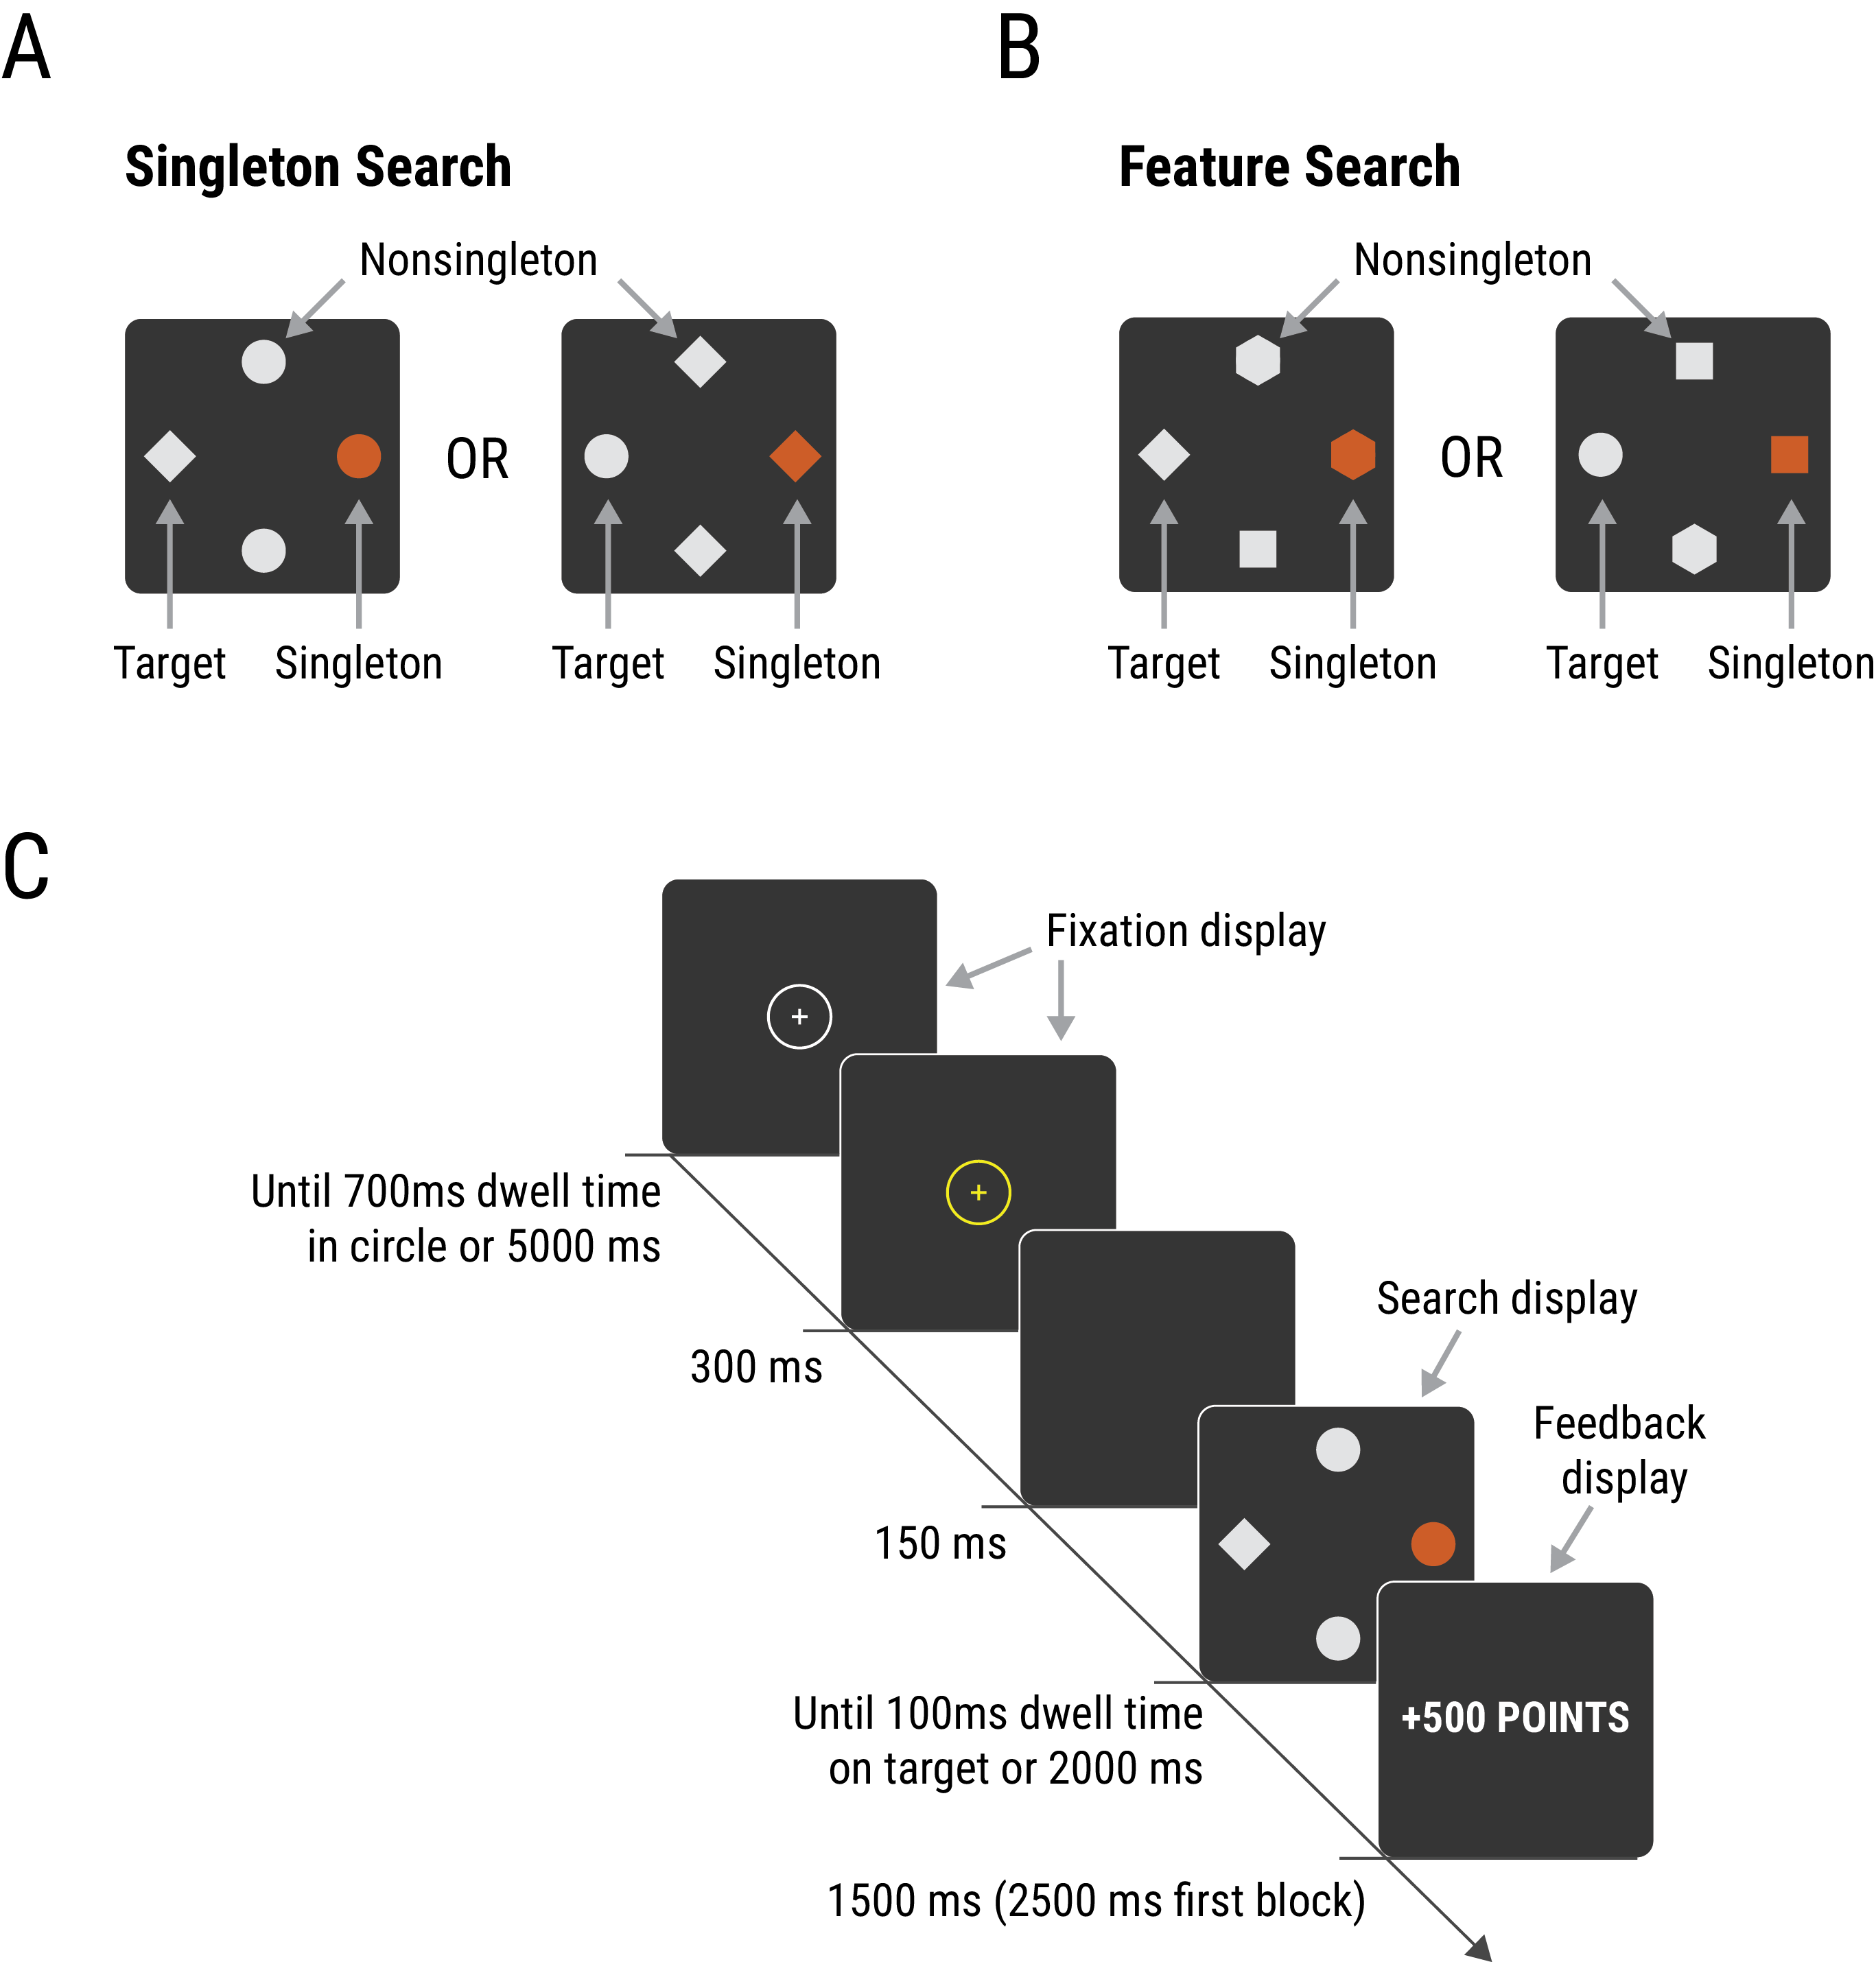
\includegraphics[width=0.8\linewidth]{C:/Users/Daniel/Google Drive/Research/vmacfeaturesearch/analysis/figures/Methods_fig} 

}

\caption{Trial structure of the current task. (A) Participants in
the singleton search condition experienced search displays where the
target was a unique shape (either a circle amongst diamonds or diamond
amongst circles). (B) Participants in the feature search condition
experienced search displays where the target was either a circle or
diamond shape presented amongst a set of heterogenous shapes. On most
trials, one of the non-target shapes was rendered in either orange or
blue so as to be a colour singleton distractor, leaving two other
nonsingleton non-targets in the display. (C) Participants began by
fixating on a centrally presented fixation cross. A search display then
appeared, and participants were required to make a rapid saccade to the
target. The colour of the singleton distractor indicated the available
reward (10 or 500 points), but looking at the distractor led to reward
omission.}\label{fig:methodFig}
\end{figure}

\subsection{Design}\label{design}

Participants were randomly assigned to either the singleton search or
feature search conditions. For half of the participants in each
condition, orange was the high-reward colour and blue was the low-reward
colour; these colour-reward relationships were reversed for the
remaining participants. There were three types of trial: (1)
\emph{high-reward trials}, in which the singleton distractor was
rendered in the high-reward colour and 500 points were available for a
rapid respnse (see below); (2) \emph{low-reward trials}, in which the
singleton distractor was rendered in the low-reward colour and 10 points
were available; and (3) \emph{distractor-absent trials}, in which all
non-targets were rendered in grey and 10 points were available. The
experiment comprised 8 blocks of 60 trials each, for a total of 480
experimental trials. Each block consisted of 20 high-reward trials, 20
low-reward trials, and 20 distractor-absent trials, in random order.
Participants took a short break between blocks.

On each trial, the location of the target was determined randomly. On
high-reward and low-reward trials, the location of the singleton
distractor was randomly selected from the three remaining locations. A
small, circular region of interest (ROI) with diameter 1.7\(^\circ\)
visual angle was defined around the centre of the target, with a larger
ROI (diameter 2.6\(^\circ\)) defined around the singleton distractor. A
response was registered when the participant had accumulated 100 ms of
gaze dwell time within the target ROI. If any gaze was detected within
the singleton ROI, the reward for the trial was not awarded (henceforth
referred to as \emph{reward omissions}). On distractor-absent trials,
one of the non-target shapes was selected at random to act as the
\enquote{singleton distractor} location. Any gaze falling within the ROI
around this (non-salient) stimulus triggered a reward omission in the
same way as on trials with a singleton distractor. Responses with RTs
that were slower than the soft-timeout threshold (1000 ms) were also not
rewarded.

\subsection{Procedure}\label{procedure}

Participants were told that their task was to move their eyes to the
target \enquote{as quickly and directly as possible} on each trial.
Those in the singleton search condition were instructed to move their
eyes to the \enquote{unique shape} on each trial, whereas those in the
feature search condition were instructed to move their eyes to the
\enquote{circle or diamond}. Participants were also informed about the
relationships between distractor colour and reward availability (e.g.,
that if an orange shape was present in the display they could 500
points, and if a blue shape was present they could win 10 points); they
were not informed that looking at the reward-associated distractor would
cancel the reward for the current trial. The instructions stated that
they would earn 0 points if their RT was slower than the soft-timeout
threshold, and that their reward also depended on how accurately they
moved their eyes to the target. Participants were told that they could
earn between 7 and 15 AUD for good performance, but no specific
information about the conversion rate from points to AUD was provided.

Each trial began with the presentation of the fixation display.
Participants' gaze location was superimposed over the display as a small
yellow dot. Once 700 ms of gaze time had accumulated within the circle
surrounding the fixation cross, or after 5000 ms, the cross and the
circle turned yellow and the dot marking the participants' gaze location
disappeared. After 300 ms the screen blanked, and after a 150 ms delay
the search display was presented until a response was recorded, or until
2000 ms (hard-timeout threshold) had passed. The feedback display then
appeared for 2500 ms during the first block, and 1500 ms in all
subsequent blocks. The inter-trial interval was 700 ms.

\subsection{Data analysis}\label{data-analysis}

In line with previous VMAC protocols (e.g., Le Pelley et al., 2015;
Pearson et al., 2016), data from the first two experimental trials, and
the first two trials after each break were discarded. Hard timeouts
(2.5\% of all trials) were also discarded. One participant was replaced
because their mean proportion of valid gaze samples during each trial
was less than 50\%. One other participant was replaced after reporting
that they had misunderstood the task instructions. For the remaining
participants, valid gaze data were registered on an average of 97.5\%
(\(SD=\) 3.7\%) of samples, suggesting high fidelity of gaze data.

Saccades were detected in the raw gaze data (sampled at 300 Hz) using a
velocity-threshold identification algorithm (Salvucci \& Goldberg,
2000). Saccade latency was measured as the duration from onset of the
search display to the point at which eye-movement velocity exceeded
40\(^\circ\)/s. Following previous protocols (Pearson et al., 2016), we
excluded trials with anticipatory saccades (saccade latency
\textless{}80 ms; 7.4\% of all trials), trials in which no gaze was
recorded within 100 pixels (5.1\(^\circ\)) of the fixation point within
the first 80 ms (4.8\% of trials), and trials in which there was
insufficient gaze data to detect a saccade (2.2\% of trials). To
classify the direction of the first saccade on each trial, the angular
deviation between the endpoint of the saccade and each stimulus location
was calculated. The saccade was defined as going in the direction of a
stimulus if the angular deviation was less than \(30^\circ\) to the left
or right of that stimulus.

There were two primary dependent measures: (1) the percentage of reward
omissions---that is, trials on which participants looked at the
singleton distractor (or nonsingleton distractor randomly assigned to
act as the \enquote{singleton distractor} location: see Design) and
hence reward was cancelled---for high-reward, low-reward, and
distractor-absent trials, and (2) the percentage of first saccades
directed towards the singleton distractor versus the average
nonsingleton distractor (that is, the mean across the two nonsingleton
distractors present in each search display; see Figure
\ref{fig:methodFig}), on high-reward and low-reward trials.

For the analysis of reward omissions, we were particularly interested in
two contrasts. First, the comparison between the high-reward and
low-reward trials allowed us to examine the effect of reward on
attention, since both displays contained a physically salient
colour-singleton distractor, with the only difference being the
magnitude of reward that the distractor signalled. Second, the
comparison between the low-reward and distractor-absent trials allowed
us to examine the effect of physical salience on attention, since these
different trial types differed in whether the display contained a
colour-singleton distractor, but had the same reward magnitude available
(10 points). These contrasts were compared for the singleton search and
feature search conditions using 2 \(\times\) 2 mixed ANOVAs.

For the analysis of saccade direction, we were primarily interested in
the difference between the percentage of trials on which first saccades
were directed towards the singleton distractor and the mean of both
nonsingleton distractors across high- and low-reward trials. These data
were converted into a \emph{capture score} by subtracting the percentage
of trials where the first saccade was directed towards the average
nonsingleton from the percentage of trials where the first saccade was
directed towards the singleton. A positive capture score indicated that
gaze was more likely to have been directed towards the singleton than
the average nonsingleton (i.e., the singleton had captured overt
attention), whereas a negative capture score indicated that gaze was
more likely to be directed toward the average nonsingleton than the
singleton (overt attention to the singleton was suppressed). A 2
\(\times\) 2 mixed ANOVA was used to compare capture scores for high-
and low-reward trials across search conditions. In addition to any group
differences in the patterns of attentional capture and/or suppression
across trial type, we were also interested in directly investigating
whether attention was captured by the singleton distractor (capture
score \(>0\)), or whether attention to the singleton was suppressed
(capture score \(<0\)) for each trial type \(\times\) search condition
combination. We therefore tested the capture score for each trial type
and search condition with planned one-sample \emph{t}-tests against
zero.

Statistical analyses were conducted in R (Version 3.5.1; R Core Team,
2018) with the afex package (Singmann, Bolker, Westfall, \& Aust, 2018)
used to calculate ANOVAs and the emmeans package (Lenth, 2018) for
follow-up contrasts. Greenhouse-Geisser corrections are reported where
appropriate. In cases where a conclusion is drawn on the basis of a null
effect, we report the Bayes factor that corresponds to a Bayesian
\emph{t}-test using the default Cauchy prior, conducted using the
BayesFactor package (Morey \& Rouder, 2018). Bayes factors are
interpreted in line with the guidelines suggested by Jeffreys (1961).
Experiment scripts, raw data, and a reproducible research compendium of
analysis scripts (Marwick, 2019) are available at
\url{https://osf.io/yrdzv/}.

\section{Results}\label{results}

\subsection{Reward Omissions}\label{reward-omissions}

Figure \ref{fig:OmissionPlot} displays the percentage of trials on which
a reward omission was triggered by the participant looking at the
singleton distractor, across search conditions and trial types, averaged
across all trial-blocks.

\begin{figure}[!h]

{\centering 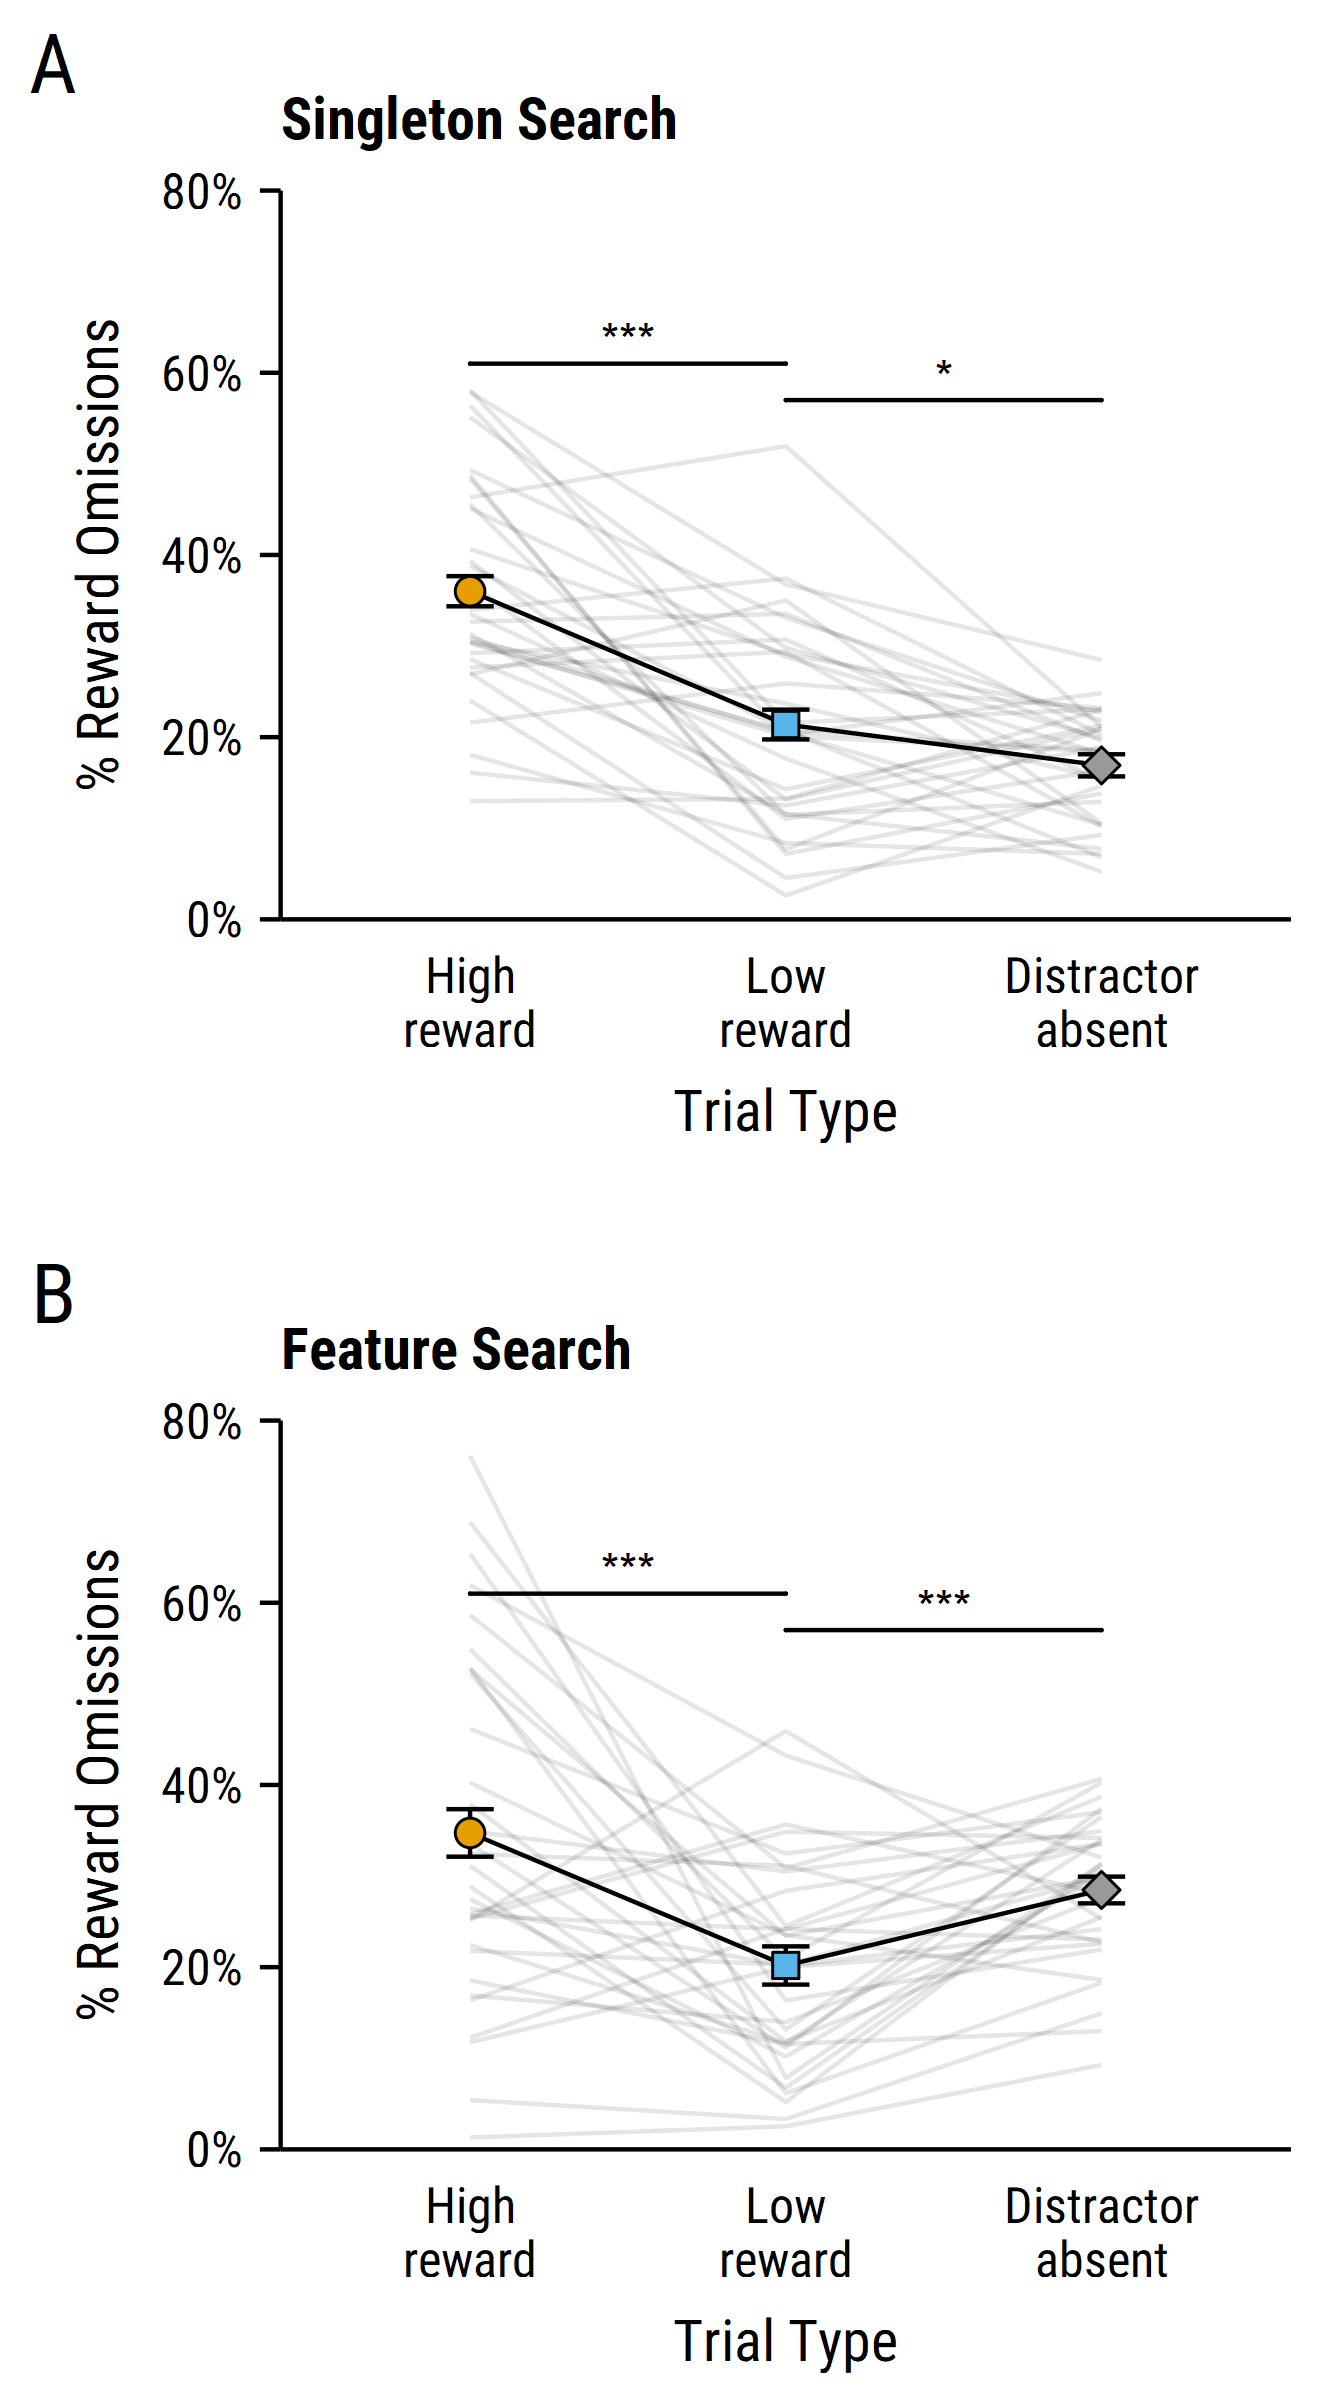
\includegraphics[width=0.6\linewidth]{C:/Users/Daniel/Google Drive/Research/vmacfeaturesearch/analysis/figures/omission_plot} 

}

\caption{Filled points show the mean percentage of reward
omissions on each trial type for the (A) singleton search condition, and
(B) feature search condition. A reward omission was triggered when the
participant looked at the singleton distractor (or the nonsingleton
distractor assigned as the \enquote{singleton} location on distractor
absent trials; see Design) prior to looking at the target. Individual
participant performance is shown by faint grey lines. Error bars in all
figures represent within-subjects SEM (Cousineau, 2005) with Morey
(2008) correction. *** \(p<.005\), * \(p<.05\).}\label{fig:OmissionPlot}
\end{figure}

\subsubsection{Effect of reward.}\label{effect-of-reward.}

ANOVA analysis of the percentage of reward omissions with factors of
trial type (high-reward vs low-reward) and search condition (singleton
search vs feature search) revealed a main effect of trial type
\(F(1, 62) = 43.11\), \(p < .001\), \(\hat{\eta}^2_p = .410\). Planned
paired-samples \emph{t}-tests confirmed that participants triggered more
reward omissions (i.e., were more likely to look at the colour-singleton
distractor) on high-reward trials than low-reward trials in both the
singleton search condition, \(t(31) = 5.87\), \(p < .001\), \(d_z=\)
1.04 (Figure \ref{fig:OmissionPlot}A) and feature search condition,
\(t(31) = 3.96\), \(p < .001\), \(d_z=\) 0.70 (Figure
\ref{fig:OmissionPlot}B), demonstrating an effect of reward on overt
attentional capture (i.e., a VMAC effect) regardless of whether
participants were encouraged to adopt a more specific target template.
Importantly, search condition did not exert a significant main effect,
\(F(1, 62) = 0.21\), \(p = .647\), \(\hat{\eta}^2_p = .003\), or
significantly interact with the effect of trial type,
\(F(1,62) < 0.01\), \(p=.985\), \(\hat{\eta}^2_p < .0001\). In order to
quantify support for the null hypothesis that the influence of reward on
attentional capture did not vary depending on participants' target
template, we conducted a Bayesian \emph{t}-test to compare the magnitude
of the VMAC effect across the two search conditions. This revealed a
Bayes Factor of \(\mathrm{BF}_{\textrm{01}} = 3.91\), indicating
moderate support for the null hypothesis of no difference in the size of
the VMAC effect under singleton search and fearure search conditions.

\subsubsection{Effect of physical
salience.}\label{effect-of-physical-salience.}

ANOVA analysis of the percentage of reward omissions revealed a
non-significant main effect of trial type (low-reward vs
distractor-absent), \(F(1, 62) = 1.83\), \(p = .181\),
\(\hat{\eta}^2_p = .029\), and a significant main effect of search
condition (singleton search vs feature search), \(F(1, 62) = 7.26\),
\(p = .009\), \(\hat{\eta}^2_p = .105\). Critically, this main effect
was qualified by a significant trial type \(\times\) search condition
interaction, \(F(1, 62) = 20.61\), \(p < .001\),
\(\hat{\eta}^2_p = .249\), indicating that the effect of physical
salience on overt attentional capture differed across search conditions.
Paired-samples \emph{t}-tests revealed that participants in the
singleton search condition triggered significantly more reward omissions
on trials that contained a colour-singleton distractor than those that
did not, \(t(31) = 2.32\), \(p = .027\), \(d_z=\) 0.41, suggesting that
overt attention was captured by the physically salient singleton. In
contrast, participants in the feature search condition triggered fewer
reward omissions on trials containing a colour-singleton distractor than
trials with no coloured singleton, \(t(31) = 4.05\), \(p < .001\),
\(d_z=\) 0.72, suggesting that overt attention to the singleton
distractor was suppressed under conditions promoting feature search,
consistent with previous findings (Gaspelin et al., 2017).

\begin{figure}[!h]

{\centering 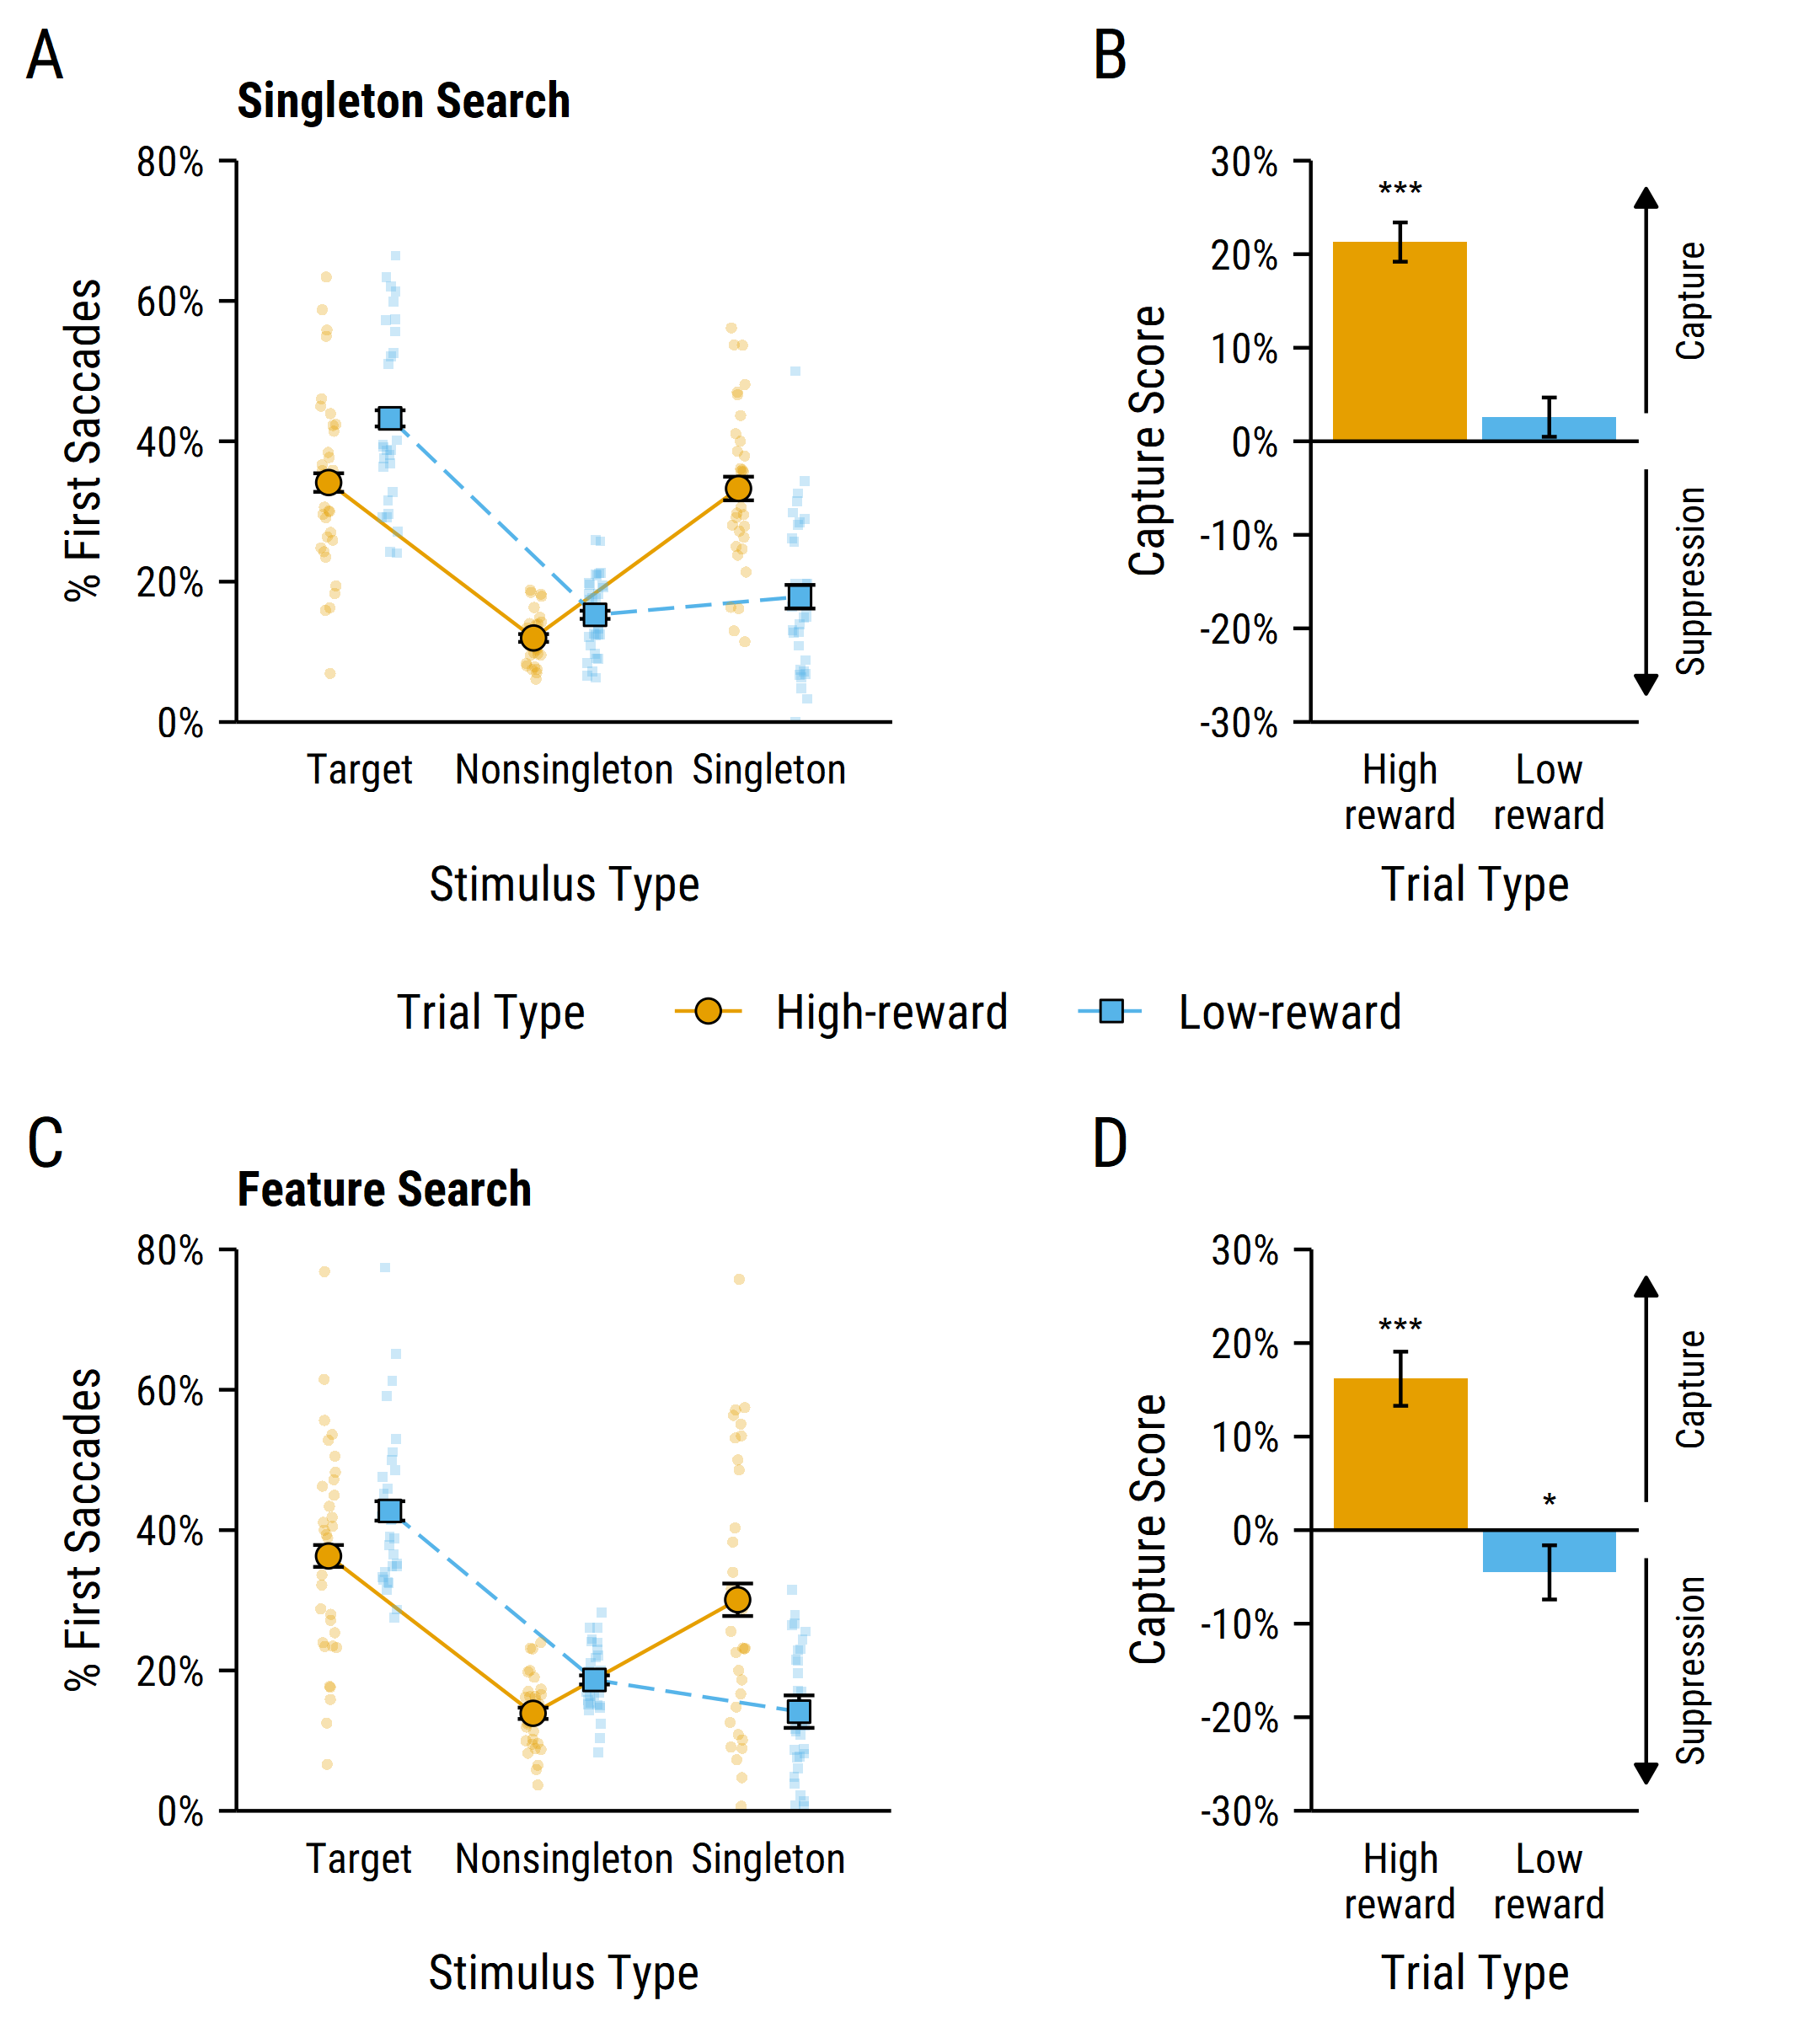
\includegraphics[width=0.8\linewidth]{C:/Users/Daniel/Google Drive/Research/vmacfeaturesearch/analysis/figures/saccade_plot} 

}

\caption{First saccade direction data. (A) Filled points show
the mean percentage of first saccades directed towards the target,
average nonsingleton distractor and singleton distractor, on high- and
low-reward trials, for participants in the singleton search condition.
Individual participant performance shown by faint underlying points. (B)
These data are converted into capture scores (calculated as the
percentage saccades to the singleton distractor minus percentage
saccades to the average nonsingleton distractor) for high-reward and
low-reward trials. Positive capture scores indicate that the singleton
distractor captured overt attention, and negative capture scores
indicate that the overt attention to the singleton distractor was
suppressed. (C) Mean percentage of first saccades to each stimulus type,
and (D) capture scores for participants in the feature search condition.
Error bars represent within-subjects SEM. *** \(p<.001\), * \(p<.05\).}\label{fig:SaccadePlot}
\end{figure}

\subsection{First Saccade Direction}\label{first-saccade-direction}

Figure \ref{fig:SaccadePlot} shows the percentage of first saccades
directed towards each stimulus type (i.e., the target\footnote{Note that
  the comparison of interest in determining whether a stimulus captured
  attention, or was suppressed, is the percentage of first saccades to
  the singleton vs.~the average nonsingleton distractor. Thus, while we
  have included the percentage of first saccades to the target in Figure
  \ref{fig:SaccadePlot} for the sake of completeness, we have not
  included these data in our analyses.}, average nonsingleton
distractor, and singleton distractor) on high- and low-reward trials for
the singleton search (Figure \ref{fig:SaccadePlot}A) and feature search
(Figure \ref{fig:SaccadePlot}C) conditions; Figures
\ref{fig:SaccadePlot}B and \ref{fig:SaccadePlot}D show capture scores
(difference in percentage of first saccades directed towards singleton
versus average nonsingleton distractor) for the singleton search and
feature search conditions, respectively. ANOVA analysis of capture
scores revealed a significant main effect of trial type (high-reward vs
low-reward), \(F(1, 62) = 45.55\), \(p < .001\),
\(\hat{\eta}^2_p = .424\), with the singleton capturing attention more
often on high-reward trials than low-reward trials; once again
demonstrating a VMAC effect. A main effect of search condition
(singleton search vs feature search), \(F(1, 62) = 4.89\), \(p = .031\),
\(\hat{\eta}^2_p = .073\), indicated that both the high-reward and
low-reward singleton captured attention more often, on average, in the
singleton search condition than the feature search condition.
Importantly, the trial type \(\times\) search condition interaction was
non-significant, \(F(1, 62) = 0.12\), \(p = .735\),
\(\hat{\eta}^2_p = .002\), with a corresponding Bayes factor of
\(\mathrm{BF}_{\textrm{01}} = 3.73\) indicating moderate support for the
null hypothesis that search condition had no effect on the magnitude of
the VMAC effect on first saccade direction.

Next we tested whether overt attention to each distractor type was
captured or suppressed in each search condition. Planned one-sample
\emph{t}-tests showed that capture scores were significantly greater
than zero (indicating that overt attention was captured by the
high-reward singleton) under conditions promoting singleton search,
\(t(31) = 9.03\), \(p < .001\), \(d_z=\) 1.60, as well as feature
search, \(t(31) = 3.98\), \(p < .001\), \(d_z=\) 0.70. For the
low-reward distractor, there was a non-significant numerical trend
towards capture in the singleton search condition, \(t(31) = 1.02\),
\(p = .313\), \(d_z=\) 0.18. In contrast, for the feature search
condition, capture score was significantly below zero, \(t(31) = 2.30\),
\(p = .028\), \(d_z=\) 0.41, indicating that overt attention to the
low-reward singleton was suppressed. Thus, in line with previous
findings (Gaspelin et al., 2017), our data suggest that overt attention
to physically salient singletons can be suppressed when participants are
encouraged to adopt a specific target template. However, singletons that
have been associated with high reward capture overt attention,
regardless of participants' target template and despite such capture
being directly counterproductive to earning reward.

\begin{figure}[!h]

{\centering 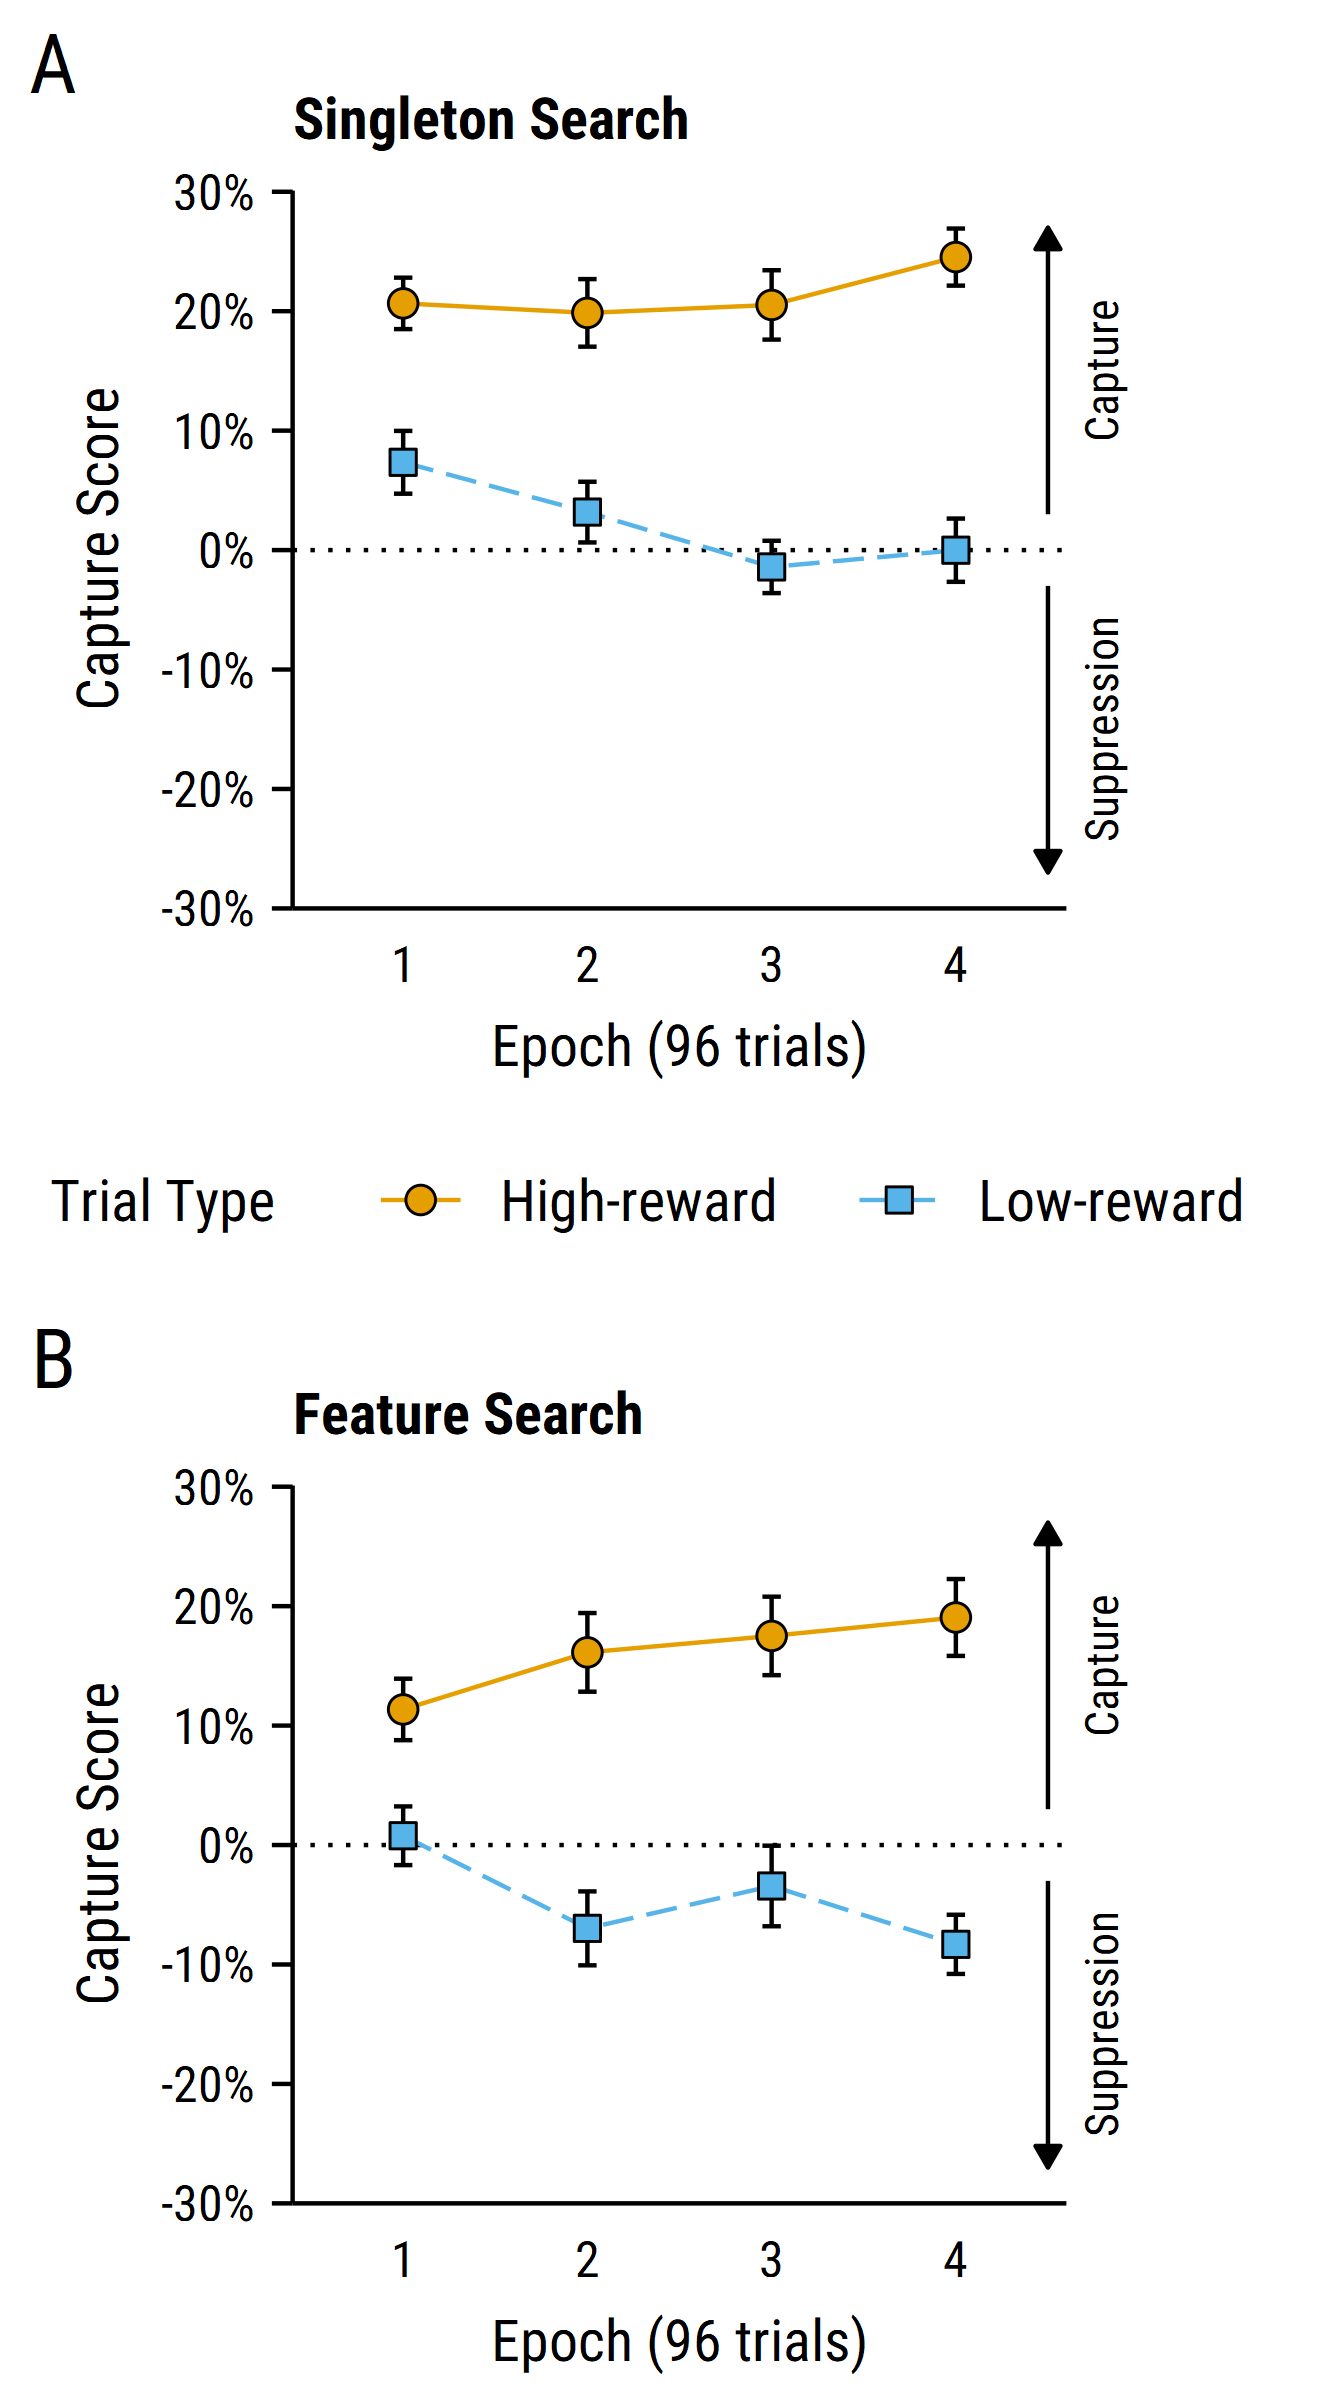
\includegraphics[width=0.6\linewidth]{C:/Users/Daniel/Google Drive/Research/vmacfeaturesearch/analysis/figures/capture_plot_by_block} 

}

\caption{Capture scores across five 96-trial epochs of the
experiment for participants in the (A) singleton search condition and
(B) feature search condition. Positive capture scores indicate that the
singleton distractor captured attention, whereas negative capture scores
indicate that attention to the singleton distractor was suppressed.
Error bars represent within-subjects SEM.}\label{fig:blockPlot}
\end{figure}

\subsection{Development of attentional capture/suppression across
training}\label{development-of-attentional-capturesuppression-across-training}

Recent research suggests that attentional suppression develops over the
course of repeated experience with the to-be-ignored stimulus feature
(Gaspelin \& Luck, 2018a; Vatterott \& Vecera, 2012). In order to
investigate this in the current study, we divided the experiment into
four epochs (96 trials/epoch) and calculated capture scores (as
described earlier) for each trial type (see Figure \ref{fig:blockPlot}).
These data were analysed using an ANOVA with factors of search condition
(singleton search, feature search), trial type (high, low), and epoch
(1--4). This once again revealed a main effect of search condition,
\(F(1, 62) = 4.97\), \(p = .029\), \(\hat{\eta}^2_p = .074\), and trial
type, \(F(1, 62) = 46.60\), \(p < .001\), \(\hat{\eta}^2_p = .429\).
Critically, there was also a significant interaction between trial type
and epoch, \(F(2.73, 169.44) = 9.77\), \(p < .001\),
\(\hat{\eta}^2_p = .136\). There were no other significant main or
interaction effects (all \emph{p}'s \(>.25\)). Follow-up contrasts
revealed a significant negative linear trend for low-reward trials,
\(t(369)=\) 4.07, \(p\) \textless{} .001, with capture by the low-reward
distractor decreasing as the experiment progressed and experience with
the physically salient feature increased (notably, in the feature search
condition scores become increasingly negative, indicating increasing
\emph{suppression} of the low-reward distractor). In contrast, for
high-reward trials there was a significant positive linear trend,
\(t(369)=\) 2.97, \(p=\) .003, with capture by the high-reward
distractor increasing as the experiment progressed and experience with
the reward associated feature increased.

\begin{figure}[!h]

{\centering 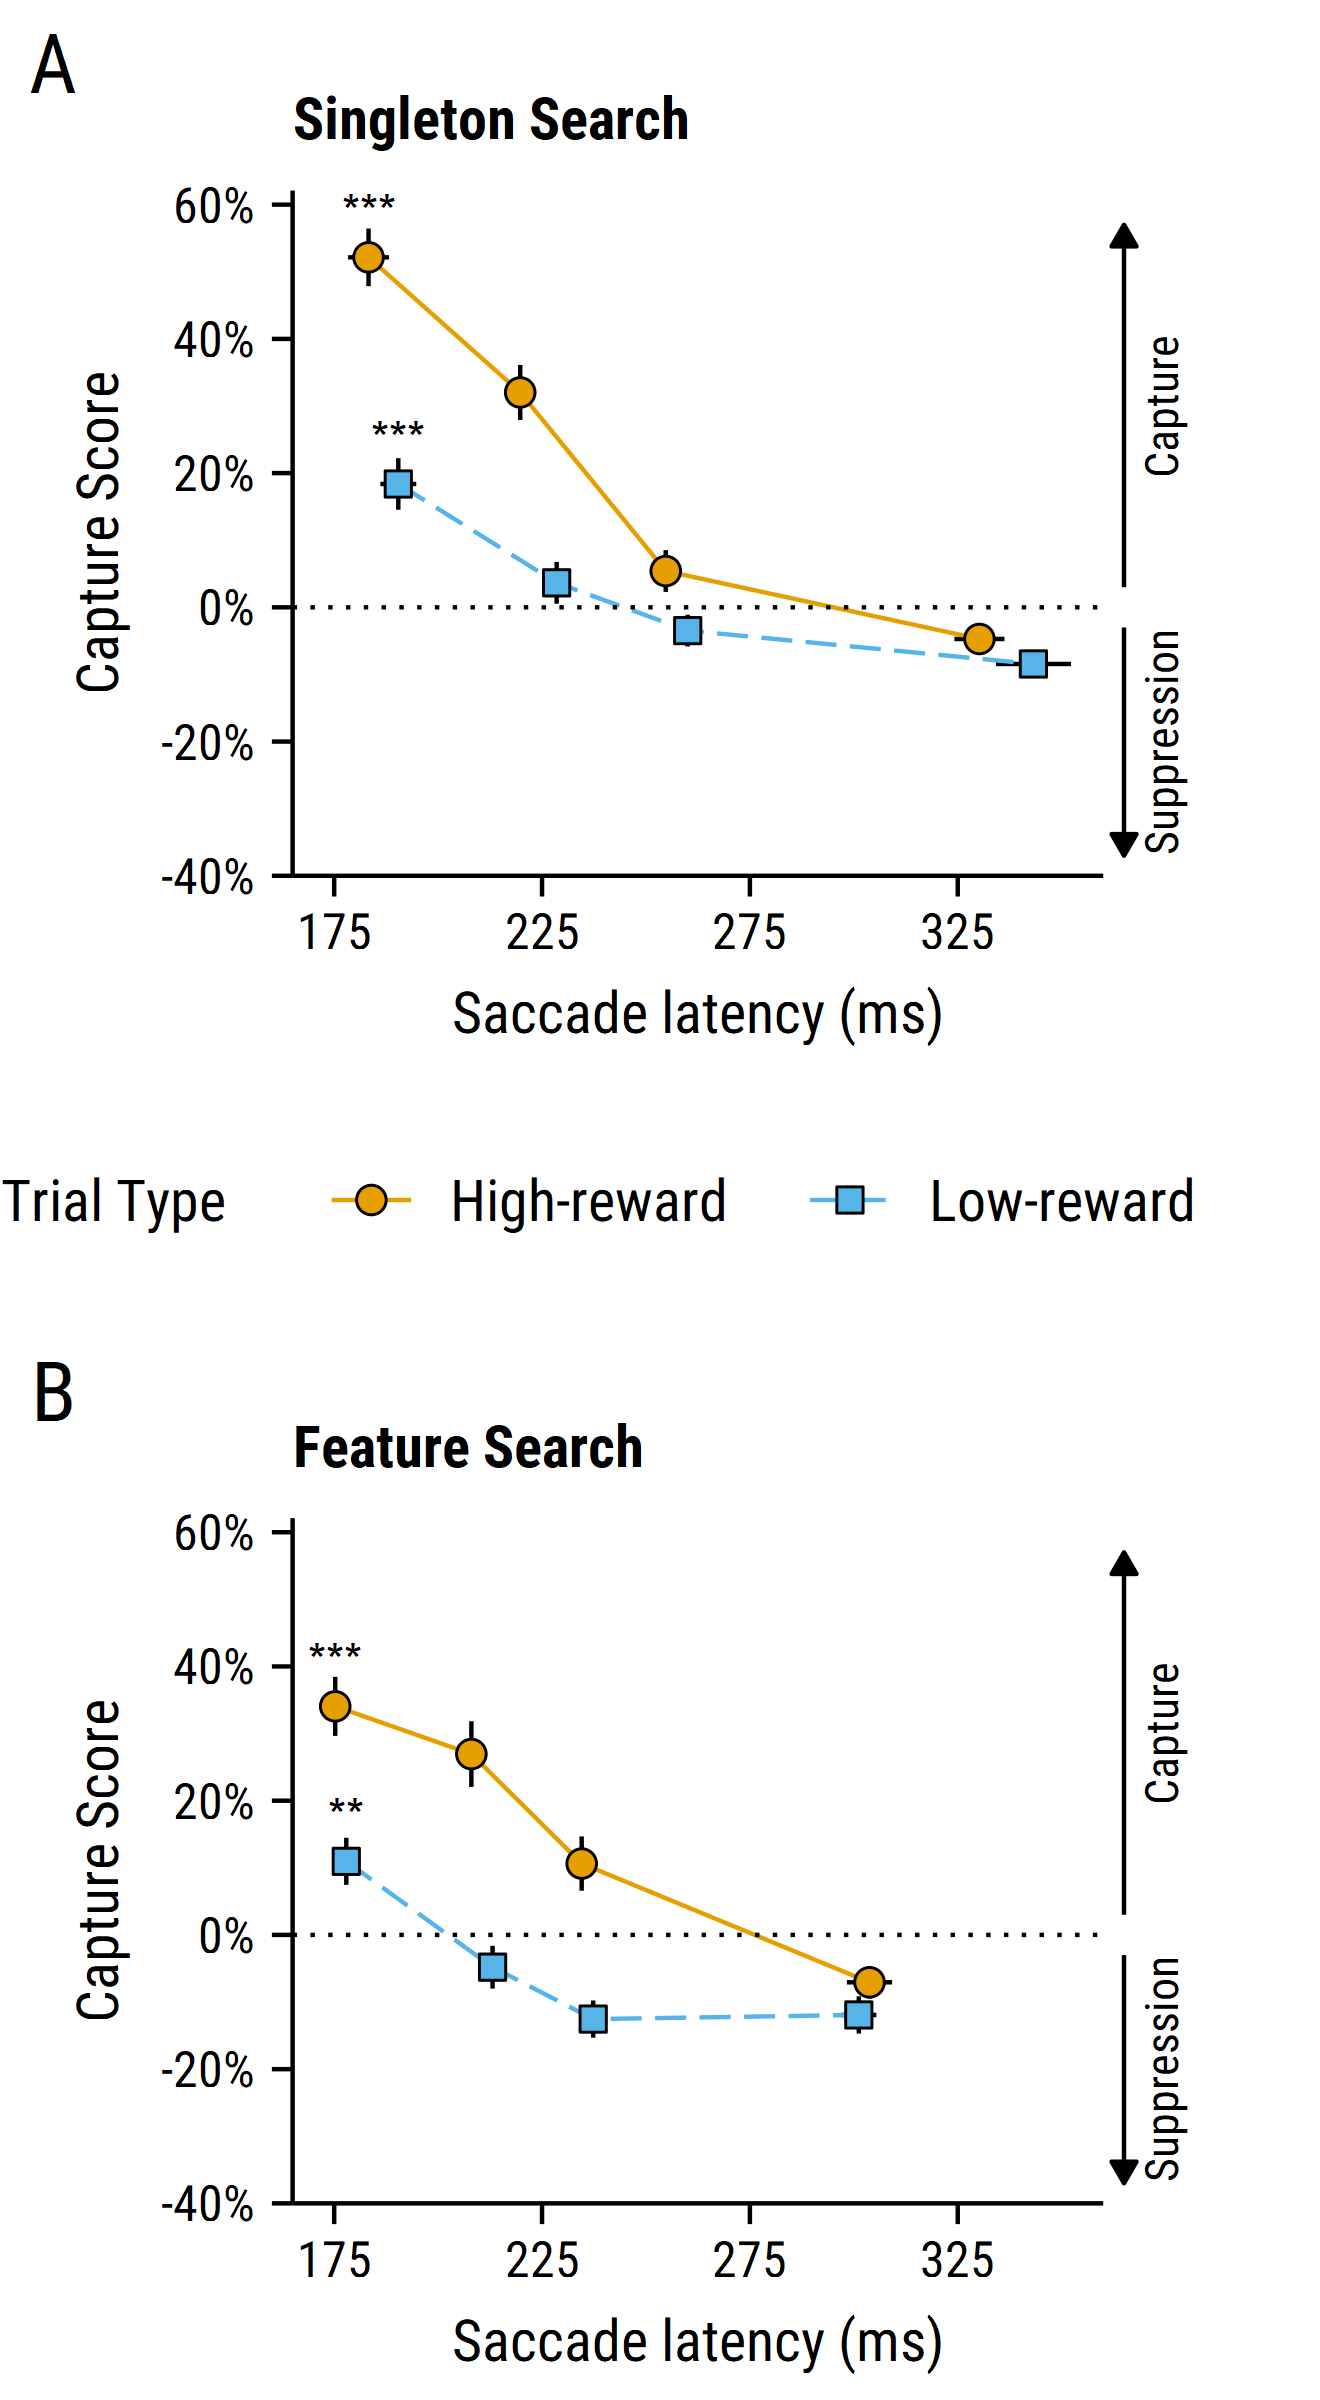
\includegraphics[width=0.6\linewidth]{C:/Users/Daniel/Google Drive/Research/vmacfeaturesearch/analysis/figures/vincentized_plot} 

}

\caption{Capture scores as a function of saccade latency
quartile for participants in the (A) singleton search condition and (B)
feature search condition. Mean first saccade latencies and the
proportion of first saccades directed towards each stimulus type were
calculated separately for each quintile of individual participant
saccade latency distributions using the Vincentizing procedure
(Ratcliff, 1979). Positive capture scores indicate that the singleton
distractor captured attention, whereas negative capture scores indicate
that attention to the singleton distractor was suppressed. Error bars
represent within-subjects SEM. *** \(p<.001\), ** \(p<.01\).}\label{fig:VincentizedPlot}
\end{figure}

\subsection{Attentional capture/suppression effects for the fastest
quartile of saccadic
latencies}\label{attentional-capturesuppression-effects-for-the-fastest-quartile-of-saccadic-latencies}

To investigate the time course of the overt attentional capture and
suppression effects, we analysed capture scores (proportion of first
saccades towards the singleton distractor minus the average nonsingleton
distractor) on high-reward and low-reward trials as a function of
saccade latency using the Vincentizing procedure (Ratcliff, 1979). We
calculated mean saccade latency and capture score separately for each
trial type and quartile of the individual saccade latency distributions.
We then analysed the capture scores for the data from the first quartile
of this distribution, i.e., the most rapidly generated saccades.
According to the signal suppression hypothesis, the attentional
suppression effect is activated early in processing, prior to the
initial allocation of attention (Gaspelin \& Luck, 2019). Therefore the
speed with which a saccade is initiated should have no effect on the
extent to which overt attention can be suppressed. As illustrated in
Figure \ref{fig:VincentizedPlot}, the most rapidly generated saccades
were captured by the high-reward singleton (capture scores \(>0\)) in
both the singleton search, \(t(31) = 13.02\), \(p < .001\), \(d_z=\)
2.30, and feature search conditions, \(t(31) = 6.45\), \(p < .001\),
\(d_z=\) 1.14. Similarly, the most rapidly generated saccades were
captured by the low-reward singleton in both the singleton search,
\(t(31) = 4.10\), \(p < .001\), \(d_z=\) 0.72, and feature search
conditions, \(t(31) = 3.34\), \(p = .002\), \(d_z=\) 0.59. It is notable
that we observed capture (rather than suppression) for the fastest
saccades for both trial-types in the feature search condition. This
finding is inconsistent with Gaspelin et al.'s (2017) previous report of
attentional suppression of physically salient singleton distractors in
the fastest eye-movements.

\section{Discussion}\label{discussion}

In this experiment, we investigated the role of inhibitory control
processes in actively suppressing overt attention to physically salient
and reward-associated distractor stimuli. In line with the signal
suppression hypothesis (Gaspelin et al., 2015, 2017), overt attention to
physically salient colour singleton distractors was suppressed under
conditions that promoted top-down guidance of attention. Specifically,
under feature search conditions, participants were generally less likely
to look at a (low-reward) colour singleton distractor than the average
nonsingleton distractor. Consistent with recent findings (Gaspelin \&
Luck, 2018a; Vatterott \& Vecera, 2012), this attentional suppression
effect gradually emerged over the course of the experiment, as
participants gained experience with the salient-but-irrelevant
distractor feature (Figure \ref{fig:blockPlot}). Furthermore, we
observed an effect of reward association on overt attention (i.e., VMAC;
Le Pelley et al., 2015; Pearson et al., 2015), with participants' gaze
more likely to be captured by distractor stimuli that signalled high
reward than low reward, even though looking at reward-signalling
distractors caused omission of rewards that otherwise would have been
delivered. Similar to the attentional suppression effect, attentional
capture by reward-associated distractors also emerged over the course of
the experiment, as participants experienced more pairings of stimulus
features with reward. Critically, this study was the first to
demonstrate that---unlike the influence of physical salience---the
influence of reward association on attention cannot be suppressed under
conditions that promote top-down guidance of attention. Regardless of
whether participants were encouraged to search for specific target
defining features (i.e., feature search mode) or to search for the
odd-one-out (singleton search mode), stimuli associated with high reward
captured overt attention. Notably, this attentional bias was
counterproductive, in that it led to the omission of more high rewards
than low rewards, and so participants should have been highly motivated
to suppress their attention to the high-reward distractor if possible.
Nevertheless, the high-reward distractor captured attention, even under
conditions that allowed participants to suppress their attention to
physically salient distractors that were associated with low reward. Our
key finding, then, is that reward-related stimuli constitute especially
potent attentional priority signals that are relatively immune to
suppression by inhibitory control processes that can act to prevent
distraction by physical salience.

Most influential models of attentional selection assume that
stimulus-driven and goal-directed influences are integrated onto a
common priority map in the brain, with attention directed towards the
spatial location with the highest peak of activation (e.g., Itti \&
Koch, 2001; Theeuwes, 2010; Wolfe, 2007). The priority map concept has
also been used to explain how selection history influences attentional
allocation (Awh et al., 2012; Failing \& Theeuwes, 2018), with the
attentional priority signal of reward-related stimulus features
increasing with repeated stimulus-reward pairings through a process of
associative learning (Le Pelley et al., 2016; Pearson et al., 2016).
Recent formulations of the signal suppression hypothesis have suggested
that the attentional suppression mechanism may operate in a similar way,
with the attentional priority of to-be-ignored stimulus features being
proactively down-weighted with repeated experience (Gaspelin \& Luck,
2019). At first glance, the results of the current study may seem
inconsistent with the idea that reward and suppression engage in
competition on a common priority map, as the magnitude of the VMAC
effect did not differ between search conditions, even though the feature
search condition should have encouraged top-down guidance of attention.
However, there was an \emph{overall} decrease in the amount of capture
by both the high- and low-reward distractor in the feature search
condition (supported by a main effect of search condition, e.g., see
Figures \ref{fig:SaccadePlot}B and \ref{fig:SaccadePlot}D). This raises
the possibility that repeated experience of the physically salient
stimulus features (i.e., orange and blue colour) allows the attentional
priority of those features to be uniformly down-weighted by the
suppression mechanism. In addition, our findings are consistent with the
idea that repeated experience of pairings between stimulus features and
reward results in selective up-weighting of the attentional priority of
the high-reward distractor, such that it overpowers the influence of
inhibitory suppression and thus captures attention.

An inconsistency between the results of the current study and those of
Gaspelin et al. (2017) comes from the time-course of the attentional
capture and suppression effects that were observed. According to the
signal suppression hypothesis, suppression is \emph{proactive}---in that
it operates prior to the initial allocation of attention---and so
suppression should be observed even for the most rapidly generated
saccades. Consistent with this idea, Gaspelin et al. (2017) observed an
overt attentional suppression effect to physically salient singleton
distractors amongst the fastest quartile of saccade latencies. By
contrast, in the current experiment we observed overt attentional
capture in the fastest quartile of saccade latencies, with the
suppression effect emerging on trials with slower saccades.
Methodological differences between Gaspelin et al.\enquote{s (2017)
experiment and the current study may be responsible for this
discrepancy. For example, the availability of reward on low-reward
trials may have influenced capture, either by somewhat increasing the
attentional priority of the stimulus feature associated with low reward,
or by otherwise influencing participants} motivation to respond quickly.
Alternatively, the discrepancy in findings may reflect our use of two
potential targets (circle and diamond) in the feature search condition,
as opposed to the same target on all trials in Gaseplin et al.'s
procedure. Having two possible targets could reduce the influence of
trial-by-trial upweighting of target features (Maljkovic \& Nakayama,
1994), but may also result in less effective feature search (but see
Grubert \& Eimer, 2015; e.g., Houtkamp \& Roelfsema, 2009). Another
possible explanation comes from the use of an intermixed trial
structure: as participants randomly experienced trials containing either
the high- or low-reward colour throughout the course of the task, it is
possible that the proactive down-weighting of the salient-but-irrelevant
features could not build up enough to prevent capture for the most
rapidly initiated saccades (Gaspelin \& Luck, 2019). How these
methodological differences might influence the time-course of overt
attentional capture and suppression remains a question for future
research. Nonetheless, the finding does raise questions about whether
the attentional suppression effect that we have observed is truly the
result of proactive attentional suppression of salient stimuli, as
suggested by the signal suppression hypothesis, or potentially the
result of rapid covert disengagement from the salient stimuli (see
Theeuwes, 2010; van Zoest et al., 2004 for similar arguments).

As mentioned previously, attentional capture by stimuli associated with
monetary rewards can be mapped on to the attentional biases to
drug-related stimuli seen in addiction. Indeed, recent findings suggest
that these biases may be the result of a common mechanism (Albertella et
al., 2017; Anderson et al., 2013). This is consistent with the idea of
incentive salience (Berridge \& Robinson, 1998), where the perceptual
representation of an otherwise neutral stimulus is modified so as to
become more salient and attention grabbing to the observer, as a result
of its association with a desired outcome (e.g., drugs, money). The
current study suggests that incentive salience has a particularly
powerful influence on the attentional system, overcoming inhibitory
control mechanisms that can effectively prevent capture by physically
salient stimuli. This may have implications for the development of
treatments for substance use disorders that target these attentional
biases.



























































\newpage

\section{References}\label{references}

\begingroup
\setlength{\parindent}{-0.5in} \setlength{\leftskip}{0.5in}

\hypertarget{refs}{}
\hypertarget{ref-Albertella2017a}{}
Albertella, L., Copeland, J., Pearson, D., Watson, P., Wiers, R. W., \&
Le Pelley, M. E. (2017). Selective attention moderates the relationship
between attentional capture by signals of nondrug reward and illicit
drug use. \emph{Drug and Alcohol Dependence}, \emph{175}, 99--105.
\url{https://doi.org/10.1016/j.drugalcdep.2017.01.041}

\hypertarget{ref-Anderson2015a}{}
Anderson, B. A. (2016). The attention habit: How reward learning shapes
attentional selection. \emph{Annals of the New York Academy of
Sciences}, \emph{1369}, 24--39. \url{https://doi.org/10.1111/nyas.12957}

\hypertarget{ref-Anderson2013}{}
Anderson, B. A., Faulkner, M. L., Rilee, J. J., Yantis, S., \& Marvel,
C. L. (2013). Attentional bias for nondrug reward is magnified in
addiction. \emph{Experimental and Clinical Psychopharmacology},
\emph{21}, 499--506. \url{https://doi.org/10.1037/a0034575}

\hypertarget{ref-Awh2012}{}
Awh, E., Belopolsky, A. V., \& Theeuwes, J. (2012). Top-down versus
bottom-up attentional control: A failed theoretical dichotomy.
\emph{Trends in Cognitive Sciences}, \emph{16}, 437--443.
\url{https://doi.org/10.1016/j.tics.2012.06.010}

\hypertarget{ref-Bacon1994}{}
Bacon, W. F., \& Egeth, H. E. (1994). Overriding stimulus-driven
attentional capture. \emph{Perception \& Psychophysics}, \emph{55},
485--496. \url{https://doi.org/10.3758/BF03205306}

\hypertarget{ref-Berridge1998}{}
Berridge, K. C., \& Robinson, T. E. (1998). What is the role of dopamine
in reward: Hedonic impact, reward learning, or incentive salience?
\emph{Brain Research Reviews}, \emph{28}, 309--369.
\url{https://doi.org/10.1016/S0165-0173(98)00019-8}

\hypertarget{ref-Brainard1997}{}
Brainard, D. H. (1997). The Psychophysics Toolbox. \emph{Spatial
Vision}, \emph{10}, 433--436.
\url{https://doi.org/10.1163/156856897X00357}

\hypertarget{ref-Cousineau2005}{}
Cousineau, D. (2005). Confidence intervals in within-subject designs: A
simpler solution to Loftus and Masson's method. \emph{Tutorials in
Quantitative Methods for Psychology}, \emph{1}, 42--45.

\hypertarget{ref-Deubel1996}{}
Deubel, H., \& Schneider, W. X. (1996). Saccade target selection and
object recognition: Evidence for a common attentional mechanism.
\emph{Vision Research}, \emph{36}, 1827--1837.
\url{https://doi.org/10.1016/0042-6989(95)00294-4}

\hypertarget{ref-Failing2018}{}
Failing, M., \& Theeuwes, J. (2018). Selection history: How reward
modulates selectivity of visual attention. \emph{Psychonomic Bulletin \&
Review}, \emph{25}, 514--538.
\url{https://doi.org/10.3758/s13423-017-1380-y}

\hypertarget{ref-Failing2015}{}
Failing, M., Nissens, T., Pearson, D., Le Pelley, M., \& Theeuwes, J.
(2015). Oculomotor capture by stimuli that signal the availability of
reward. \emph{Journal of Neurophysiology}, \emph{114}, 2316--2327.
\url{https://doi.org/10.1152/jn.00441.2015}

\hypertarget{ref-Faul2007}{}
Faul, F., Erdfelder, E., Lang, A.-G., \& Buchner, A. (2007). G*Power 3:
A flexible statistical power analysis program for the social,
behavioral, and biomedical sciences. \emph{Behavior Research Methods},
\emph{39}, 175--191. \url{https://doi.org/10.3758/BF03193146}

\hypertarget{ref-Field2008}{}
Field, M., \& Cox, W. M. (2008). Attentional bias in addictive
behaviors: A review of its development, causes, and consequences.
\emph{Drug and Alcohol Dependence}, \emph{97}, 1--20.
\url{https://doi.org/10.1016/j.drugalcdep.2008.03.030}

\hypertarget{ref-Folk1992}{}
Folk, C. L., Remington, R. W., \& Johnston, J. C. (1992). Involuntary
covert orienting is contingent on attentional control settings.
\emph{Journal of Experimental Psychology. Human Perception and
Performance}, \emph{18}, 1030--1044.
\url{https://doi.org/10.1037/0096-1523.18.4.1030}

\hypertarget{ref-Gaspelin2018b}{}
Gaspelin, N., \& Luck, S. J. (2018a). Distinguishing among potential
mechanisms of singleton suppression. \emph{Journal of Experimental
Psychology: Human Perception and Performance}, \emph{44}, 626--644.
\url{https://doi.org/10.1037/xhp0000484}

\hypertarget{ref-Gaspelin2018}{}
Gaspelin, N., \& Luck, S. J. (2018b). The role of inhibition in avoiding
distraction by salient stimuli. \emph{Trends in Cognitive Sciences},
\emph{22}, 79--92. \url{https://doi.org/10.1016/j.tics.2017.11.001}

\hypertarget{ref-Gaspelin2018a}{}
Gaspelin, N., \& Luck, S. J. (2019). Inhibition as a potential
resolution to the attentional capture debate. \emph{Current Opinion in
Psychology}, \emph{29}, 12--18.
\url{https://doi.org/10.1016/j.copsyc.2018.10.013}

\hypertarget{ref-Gaspelin2015}{}
Gaspelin, N., Leonard, C. J., \& Luck, S. J. (2015). Direct evidence for
active suppression of salient-but-irrelevant sensory inputs.
\emph{Psychological Science}, \emph{26}, 1740--1750.
\url{https://doi.org/10.1177/0956797615597913}

\hypertarget{ref-Gaspelin2016}{}
Gaspelin, N., Leonard, C. J., \& Luck, S. J. (2017). Suppression of
overt attentional capture by salient-but-irrelevant color singletons.
\emph{Attention, Perception, \& Psychophysics}, \emph{79}, 45--62.
\url{https://doi.org/10.3758/s13414-016-1209-1}

\hypertarget{ref-Grubert2015}{}
Grubert, A., \& Eimer, M. (2015). Rapid parallel attentional target
selection in single-color and multiple-color visual search.
\emph{Journal of Experimental Psychology: Human Perception and
Performance}, \emph{41}, 86--101.
\url{https://doi.org/10.1037/xhp0000019}

\hypertarget{ref-Hickey2010}{}
Hickey, C., Chelazzi, L., \& Theeuwes, J. (2010). Reward changes
salience in human vision via the anterior cingulate. \emph{Journal of
Neuroscience}, \emph{30}, 11096--11103.
\url{https://doi.org/10.1523/JNEUROSCI.1026-10.2010}

\hypertarget{ref-Houtkamp2009}{}
Houtkamp, R., \& Roelfsema, P. R. (2009). Matching of visual input to
only one item at any one time. \emph{Psychological Research}, \emph{73},
317--326. \url{https://doi.org/10.1007/s00426-008-0157-3}

\hypertarget{ref-Ipata2006}{}
Ipata, A. E., Gee, A. L., Gottlieb, J., Bisley, J. W., \& Goldberg, M.
E. (2006). LIP responses to a popout stimulus are reduced if it is
overtly ignored. \emph{Nature Neuroscience}, \emph{9}, 1071--1076.
\url{https://doi.org/10.1038/nn1734}

\hypertarget{ref-Itti2001}{}
Itti, L., \& Koch, C. (2001). Computational modelling of visual
attention. \emph{Nature Reviews Neuroscience}, \emph{2}, 194--203.
\url{https://doi.org/10.1038/35058500}

\hypertarget{ref-Jeffreys1961}{}
Jeffreys, H. (1961). \emph{Theory of probability} (3rd ed.). Oxford, UK:
Oxford University Press.

\hypertarget{ref-Kleiner2007}{}
Kleiner, M., Brainard, D. H., Pelli, D. G., Broussard, C., Wolf, T., \&
Niehorster, D. (2007). What's new in Psychtoolbox-3? \emph{Perception},
\emph{36}, S14. \url{https://doi.org/10.1068/v070821}

\hypertarget{ref-LePelleya}{}
Le Pelley, M. E., Mitchell, C. J., Beesley, T., George, D. N., \& Wills,
A. J. (2016). Attention and associative learning in humans: An
integrative review. \emph{Psychological Bulletin}, \emph{142},
1111--1140. \url{https://doi.org/10.1037/bul0000064}

\hypertarget{ref-LePelley2015b}{}
Le Pelley, M. E., Pearson, D., Griffiths, O., \& Beesley, T. (2015).
When goals conflict with values: Counterproductive attentional and
oculomotor capture by reward-related stimuli. \emph{Journal of
Experimental Psychology: General}, \emph{144}, 158--171.
\url{https://doi.org/10.1037/xge0000037}

\hypertarget{ref-Leber2006}{}
Leber, A. B., \& Egeth, H. E. (2006). It's under control: Top-down
search strategies can override attentional capture. \emph{Psychonomic
Bulletin \& Review}, \emph{13}, 132--138.
\url{https://doi.org/10.3758/BF03193824}

\hypertarget{ref-R-emmeans}{}
Lenth, R. (2018). \emph{Emmeans: Estimated marginal means, aka
least-squares means}. Retrieved from
\url{https://CRAN.R-project.org/package=emmeans}

\hypertarget{ref-Maljkovic1994}{}
Maljkovic, V., \& Nakayama, K. (1994). Priming of pop-out: I. Role of
features. \emph{Memory \& Cognition}, \emph{22}, 657--672.
\url{https://doi.org/10.3758/BF03209251}

\hypertarget{ref-Marhe2013}{}
Marhe, R., Waters, A. J., Wetering, B. J. M. van de, \& Franken, I. H.
A. (2013). Implicit and explicit drug-related cognitions during
detoxification treatment are associated with drug relapse: An ecological
momentary assessment study. \emph{Journal of Consulting and Clinical
Psychology}, \emph{81}, 1--12. \url{https://doi.org/10.1037/a0030754}

\hypertarget{ref-Marissen2006}{}
Marissen, M. A. E., Franken, I. H. A., Waters, A. J., Blanken, P., Van
Den Brink, W., \& Hendriks, V. M. (2006). Attentional bias predicts
heroin relapse following treatment. \emph{Addiction}, \emph{101},
1306--1312. \url{https://doi.org/10.1111/j.1360-0443.2006.01498.x}

\hypertarget{ref-R-rrtools}{}
Marwick, B. (2019). \emph{Rrtools: Creates a reproducible research
compendium}. Retrieved from \url{https://github.com/benmarwick/rrtools}

\hypertarget{ref-Morey2008}{}
Morey, R. D. (2008). Confidence intervals from normalized data: A
correction to Cousineau (2005). \emph{Tutorials in Quantitative Methods
for Psychology}, \emph{4}, 61--64.
\url{https://doi.org/10.3758/s13414-012-0291-2}

\hypertarget{ref-R-BayesFactor}{}
Morey, R. D., \& Rouder, J. N. (2018). \emph{BayesFactor: Computation of
bayes factors for common designs}. Retrieved from
\url{https://CRAN.R-project.org/package=BayesFactor}

\hypertarget{ref-Pearson2015}{}
Pearson, D., Donkin, C., Tran, S. C., Most, S. B., \& Le Pelley, M. E.
(2015). Cognitive control and counterproductive oculomotor capture by
reward-related stimuli. \emph{Visual Cognition}, \emph{23}, 41--66.
\url{https://doi.org/10.1080/13506285.2014.994252}

\hypertarget{ref-Pearson2016}{}
Pearson, D., Osborn, R., Whitford, T. J., Failing, M., Theeuwes, J., \&
Le Pelley, M. E. (2016). Value-modulated oculomotor capture by
task-irrelevant stimuli is a consequence of early competition on the
saccade map. \emph{Attention, Perception, \& Psychophysics}, \emph{78},
2226--2240. \url{https://doi.org/10.3758/s13414-016-1135-2}

\hypertarget{ref-Pelli1997}{}
Pelli, D. G. (1997). The VideoToolbox software for visual psychophysics:
Transforming numbers into movies. \emph{Spatial Vision}, \emph{10},
437--442. \url{https://doi.org/10.1163/156856897X00366}

\hypertarget{ref-R-base}{}
R Core Team. (2018). \emph{R: A language and environment for statistical
computing}. Vienna, Austria: R Foundation for Statistical Computing.
Retrieved from \url{https://www.R-project.org/}

\hypertarget{ref-Ratcliff1979}{}
Ratcliff, R. (1979). Group reaction time distributions and an analysis
of distribution statistics. \emph{Psychological Bulletin}, \emph{86},
446--461. \url{https://doi.org/10.1037/0033-2909.86.3.446}

\hypertarget{ref-Salvucci2000}{}
Salvucci, D. D., \& Goldberg, J. H. (2000). Identifying fixations and
saccades in eye-tracking protocols. In \emph{Proceedings of the
symposium on eye tracking research \& applications - etra '00} (pp.
71--78). New York, NY: ACM Press.
\url{https://doi.org/10.1145/355017.355028}

\hypertarget{ref-Sawaki2010}{}
Sawaki, R., \& Luck, S. J. (2010). Capture versus suppression of
attention by salient singletons: Electrophysiological evidence for an
automatic attend-to-me signal. \emph{Attention, Perception, \&
Psychophysics}, \emph{72}, 1455--1470.

\hypertarget{ref-R-afex}{}
Singmann, H., Bolker, B., Westfall, J., \& Aust, F. (2018). \emph{Afex:
Analysis of factorial experiments}. Retrieved from
\url{https://CRAN.R-project.org/package=afex}

\hypertarget{ref-Theeuwes1991a}{}
Theeuwes, J. (1991). Cross-dimensional perceptual selectivity.
\emph{Perception \& Psychophysics}, \emph{50}, 184--193.
\url{https://doi.org/10.3758/BF03212219}

\hypertarget{ref-Theeuwes1992}{}
Theeuwes, J. (1992). Perceptual selectivity for color and form.
\emph{Perception \& Psychophysics}, \emph{51}, 599--606.
\url{https://doi.org/10.3758/BF03211656}

\hypertarget{ref-Theeuwes2010}{}
Theeuwes, J. (2010). Top-down and bottom-up control of visual selection.
\emph{Acta Psychologica}, \emph{135}, 77--99.
\url{https://doi.org/10.1016/j.actpsy.2010.02.006}

\hypertarget{ref-VanZoest2004}{}
van Zoest, W., Donk, M., \& Theeuwes, J. (2004). The role of
stimulus-driven and goal-driven control in saccadic visual selection.
\emph{Journal of Experimental Psychology: Human Perception and
Performance}, \emph{30}, 746--759.
\url{https://doi.org/10.1037/0096-1523.30.4.749}

\hypertarget{ref-Vatterott2012}{}
Vatterott, D. B., \& Vecera, S. P. (2012). Experience-dependent
attentional tuning of distractor rejection. \emph{Psychonomic Bulletin
\& Review}, \emph{19}, 871--878.
\url{https://doi.org/10.3758/s13423-012-0280-4}

\hypertarget{ref-Waters2012}{}
Waters, A. J., Marhe, R., \& Franken, I. H. A. (2012). Attentional bias
to drug cues is elevated before and during temptations to use heroin and
cocaine. \emph{Psychopharmacology}, \emph{219}, 909--921.
\url{https://doi.org/10.1007/s00213-011-2424-z}

\hypertarget{ref-Watson2019}{}
Watson, P., Pearson, D., Wiers, R. W., \& Le Pelley, M. E. (2019).
Prioritizing pleasure and pain: Attentional capture by reward-related
and punishment-related stimuli. \emph{Current Opinion in Behavioral
Sciences}, \emph{26}, 107--113.
\url{https://doi.org/10.1016/j.cobeha.2018.12.002}

\hypertarget{ref-Wolfe2007}{}
Wolfe, J. M. (2007). Guided search 4.0. In \emph{Integrated models of
cognitive systems} (pp. 99--119). Oxford University Press.
\url{https://doi.org/10.1093/acprof:oso/9780195189193.003.0008}

\hypertarget{ref-Yantis2000}{}
Yantis, S. (2000). Goal-directed and stimulus-driven determinants of
attentional control. In S. Monsell \& J. Driver (Eds.), \emph{Control of
cognitive processes: Attention and performance xvii} (pp. 73--103).
Cambridge, MA: MIT Press.

\endgroup


\end{document}
